% lauritzen_ma_datasheet_conversion_it.tex
% Dai dati del datasheet al modello di diodo di Lauritzen-Ma: teoria e regole di conversione.
% Versione italiana di lauritzen_ma_datasheet_conversion.tex (stessa struttura, stesse etichette, stesse equazioni).
% Template pwr-control (AAA_template_latex_settings); numeri e figure degli esempi svolti:
% lm_conversion_calc.py (con il modulo lm_conversion.py), che scrive lm_conversion_values.tex e figures/fig_*_it.pdf
% Compilazione: pdflatex lauritzen_ma_datasheet_conversion_it.tex  (due volte, per i riferimenti)
% Rev. 00 - novembre 2026 - prima emissione
\documentclass[10pt,a4paper]{scrartcl}
\PassOptionsToPackage{main=italian}{babel}   % settings.tex carica babel con [british]: l'italiano diventa la lingua principale
\input{../../../../AAA_template_latex_settings/settings}
% il documento sta quattro livelli sotto la radice del repository: percorso del logo di settings.tex corretto qui
\rhead{\includegraphics[height=0.75cm]{../../../../AAA_template_latex_settings/pwr-control_logo_doc.png}}
\rfoot{\small Rev.~00}
\geometry{left=2.0cm, right=2.0cm}
\usepackage[european resistors, american inductors]{circuitikz}
\usepackage{icomma}   % virgola decimale nelle formule: 0,35 senza lo spazio della punteggiatura
\babelhyphenation[italian]{data-sheet soft-ness}   % prestiti inglesi

\sisetup{output-decimal-marker={,},per-mode=symbol,range-phrase={\text{--}},range-units=single}
\setlist{nosep}
\setlength{\parindent}{0pt}
\setlength{\parskip}{3pt}
\allowdisplaybreaks
\captionsetup{font=small,labelfont=bf}
\renewcommand{\topfraction}{0.9}
\renewcommand{\bottomfraction}{0.9}
\renewcommand{\textfraction}{0.05}
\renewcommand{\floatpagefraction}{0.8}

% --- numeri degli esempi svolti (generati da lm_conversion_calc.py) ---
% Lo stesso file della versione inglese, letto sostituendo il punto decimale con la virgola: ogni macro \lm...
% si espande in un numero come 1,879, valido sia nel testo sia dentro \SI{}{} e \num{} di siunitx.
\ExplSyntaxOn
\cs_new_protected:Npn \lmitdefine #1#2
  {
    \tl_set:Nn \l_tmpa_tl {#2}
    \tl_replace_all:Nnn \l_tmpa_tl { . } { , }
    \cs_gset_eq:NN #1 \l_tmpa_tl
  }
\ExplSyntaxOff
\begingroup
\let\newcommand\lmitdefine
% generated by lm_conversion_calc.py: do not edit by hand
\newcommand{\lmKLine}{1.879}
\newcommand{\lmKTen}{2.303}
\newcommand{\lmKQuarter}{1.386}
\newcommand{\lmKLineHalf}{0.94}
\newcommand{\lmKLineLossPct}{6}
\newcommand{\lmKTenGainPct}{15}
\newcommand{\lmKSpread}{0.92}
\newcommand{\lmTEndTaus}{3.9}
\newcommand{\lmPEndPct}{2}
\newcommand{\lmTailFrac}{0.98}
\newcommand{\lmSofStretchThree}{1.74}
\newcommand{\lmFDefTwo}{13.5}
\newcommand{\lmQDefLoTwo}{17.4}
\newcommand{\lmQDefHiTwo}{23.1}
\newcommand{\lmFDefThree}{5.0}
\newcommand{\lmQDefLoThree}{6.6}
\newcommand{\lmQDefHiThree}{8.8}
\newcommand{\lmFDefFour}{1.8}
\newcommand{\lmQDefLoFour}{2.4}
\newcommand{\lmQDefHiFour}{3.3}
\newcommand{\lmFDefFive}{0.7}
\newcommand{\lmQDefLoFive}{0.9}
\newcommand{\lmQDefHiFive}{1.2}
\newcommand{\lmXLong}{3}
\newcommand{\lmQfracRhoLo}{48}
\newcommand{\lmSofRhoLo}{0.50}
\newcommand{\lmQfracRhoMid}{44}
\newcommand{\lmSofRhoMid}{1.08}
\newcommand{\lmQfracRhoHi}{38}
\newcommand{\lmSofRhoHi}{2.00}
\newcommand{\lmTenthErrTwo}{0.6}
\newcommand{\lmTenthErrFour}{3.1}
\newcommand{\lmRatioLoOne}{0.08}
\newcommand{\lmRatioHiOne}{0.21}
\newcommand{\lmRatioOneHalf}{0.21}
\newcommand{\lmRatioOneOne}{0.17}
\newcommand{\lmRatioOneTwo}{0.12}
\newcommand{\lmRatioOneFour}{0.08}
\newcommand{\lmRatioLoFive}{0.12}
\newcommand{\lmRatioHiFive}{0.36}
\newcommand{\lmRatioFiveHalf}{0.36}
\newcommand{\lmRatioFiveOne}{0.28}
\newcommand{\lmRatioFiveTwo}{0.20}
\newcommand{\lmRatioFiveFour}{0.12}
\newcommand{\lmSensTrrQHalf}{3.0}
\newcommand{\lmSensTrrIHalf}{5.0}
\newcommand{\lmSensTrrAHalf}{2.0}
\newcommand{\lmSensTauQHalf}{0.60}
\newcommand{\lmSensTauIHalf}{0.20}
\newcommand{\lmSensTauAHalf}{0.40}
\newcommand{\lmSensTmQHalf}{3.6}
\newcommand{\lmSensTmIHalf}{6.2}
\newcommand{\lmSensTmAHalf}{2.6}
\newcommand{\lmSensTrrQOne}{2.0}
\newcommand{\lmSensTrrIOne}{3.0}
\newcommand{\lmSensTrrAOne}{1.0}
\newcommand{\lmSensTauQOne}{0.67}
\newcommand{\lmSensTauIOne}{0.33}
\newcommand{\lmSensTauAOne}{0.33}
\newcommand{\lmSensTmQOne}{2.7}
\newcommand{\lmSensTmIOne}{4.3}
\newcommand{\lmSensTmAOne}{1.7}
\newcommand{\lmSensTrrQTwo}{1.5}
\newcommand{\lmSensTrrITwo}{2.0}
\newcommand{\lmSensTrrATwo}{0.5}
\newcommand{\lmSensTauQTwo}{0.75}
\newcommand{\lmSensTauITwo}{0.50}
\newcommand{\lmSensTauATwo}{0.25}
\newcommand{\lmSensTmQTwo}{2.3}
\newcommand{\lmSensTmITwo}{3.5}
\newcommand{\lmSensTmATwo}{1.3}
\newcommand{\lmAIf}{1000}
\newcommand{\lmASlope}{5}
\newcommand{\lmAIrr}{125}
\newcommand{\lmAQrr}{3200}
\newcommand{\lmAVr}{100}
\newcommand{\lmAT}{150}
\newcommand{\lmAVrrm}{4500}
\newcommand{\lmAVrrmKv}{4.5}
\newcommand{\lmAIrrmMa}{50}
\newcommand{\lmATa}{25.0}
\newcommand{\lmAQtri}{1563}
\newcommand{\lmAQtriPct}{49}
\newcommand{\lmAQoverI}{25.6}
\newcommand{\lmATaHalf}{12.5}
\newcommand{\lmATrr}{13.1}
\newcommand{\lmAS}{1.05}
\newcommand{\lmATau}{38.2}
\newcommand{\lmATm}{19.9}
\newcommand{\lmATauL}{38.1}
\newcommand{\lmATmL}{20.0}
\newcommand{\lmARho}{0.34}
\newcommand{\lmATmOverTau}{0.52}
\newcommand{\lmASoftLong}{1.05}
\newcommand{\lmAIrrOverIf}{0.125}
\newcommand{\lmALam}{5.24}
\newcommand{\lmAX}{5.89}
\newcommand{\lmAF}{0.997}
\newcommand{\lmATone}{225}
\newcommand{\lmATzero}{200}
\newcommand{\lmAIter}{7}
\newcommand{\lmATauLErr}{-0.2}
\newcommand{\lmATmLErr}{+0.1}
\newcommand{\lmAIrrBackL}{124.7}
\newcommand{\lmAQrrBackL}{3187}
\newcommand{\lmAIrrBackLErr}{-0.3}
\newcommand{\lmAQrrBackLErr}{-0.4}
\newcommand{\lmAQzero}{7246}
\newcommand{\lmAQzeroPct}{44}
\newcommand{\lmAQstat}{38169}
\newcommand{\lmATrrNinetyEight}{13.4}
\newcommand{\lmATauNinetyEight}{38.4}
\newcommand{\lmATmNinetyEight}{20.5}
\newcommand{\lmAExpIa}{0.99}
\newcommand{\lmAExpQa}{0.98}
\newcommand{\lmAExpIf}{0.01}
\newcommand{\lmAExpQf}{0.02}
\newcommand{\lmANumErr}{6\times10^{-9}}
\newcommand{\lmAIsSecOne}{2.2\times10^{-8}}
\newcommand{\lmARsSecOne}{0.560}
\newcommand{\lmAIsTanOne}{2.8\times10^{-8}}
\newcommand{\lmARsTanOne}{0.564}
\newcommand{\lmAIsSecTwo}{2.5\times10^{-3}}
\newcommand{\lmARsSecTwo}{0.520}
\newcommand{\lmAIsTanTwo}{3.2\times10^{-3}}
\newcommand{\lmARsTanTwo}{0.527}
\newcommand{\lmAVt}{36.46}
\newcommand{\lmAVto}{0.85}
\newcommand{\lmARt}{0.60}
\newcommand{\lmAIone}{500}
\newcommand{\lmAItwo}{1500}
\newcommand{\lmAN}{2}
\newcommand{\lmANmaxSec}{15.0}
\newcommand{\lmANmaxTan}{16.5}
\newcommand{\lmASlopeJct}{0.073}
\newcommand{\lmAVfLine}{1.45}
\newcommand{\lmAVlow}{0.82}
\newcommand{\lmAVlowLine}{0.91}
\newcommand{\lmAVlowDiff}{85}
\newcommand{\lmAVlowOne}{0.87}
\newcommand{\lmAIsStar}{3.8\times10^{-3}}
\newcommand{\lmAIsFactor}{1.52}
\newcommand{\lmAIsOffsetMv}{31}
\newcommand{\lmARr}{90}
\newcommand{\lmADcm}{12}
\newcommand{\lmALdiff}{214}
\newcommand{\lmAWpar}{536}
\newcommand{\lmAWmode}{486}
\newcommand{\lmAWstat}{565}
\newcommand{\lmADoverL}{1.32}
\newcommand{\lmATrrLine}{49.6}
\newcommand{\lmATrrTen}{55.2}
\newcommand{\lmATrrTri}{51.2}
\newcommand{\lmAStretch}{2.21}
\newcommand{\lmASLine}{0.98}
\newcommand{\lmASlopeRatio}{0.52}
\newcommand{\lmAQoverIf}{3.20}
\newcommand{\lmATauIfRatio}{11.9}
\newcommand{\lmAIrrFast}{1914}
\newcommand{\lmAQrrFast}{25069}
\newcommand{\lmAL}{20.0}
\newcommand{\lmAVpk}{291}
\newcommand{\lmAErec}{320}
\newcommand{\lmAOvFactor}{2.91}
\newcommand{\lmASensTauQ}{+0.68}
\newcommand{\lmASensTauI}{-0.35}
\newcommand{\lmASensTauA}{-0.32}
\newcommand{\lmASensTauF}{-0.01}
\newcommand{\lmASensTmQ}{+2.62}
\newcommand{\lmASensTmI}{-4.25}
\newcommand{\lmASensTmA}{+1.62}
\newcommand{\lmASensTmF}{+0.01}
\newcommand{\lmASensTrrQ}{+1.95}
\newcommand{\lmASensTrrI}{-2.91}
\newcommand{\lmASensTrrA}{+0.95}
\newcommand{\lmASensTrrF}{+0.00}
\newcommand{\lmAFiveTau}{-1.6}
\newcommand{\lmAFiveTm}{-19}
\newcommand{\lmAFiveTrr}{-14}
\newcommand{\lmACj}{20}
\newcommand{\lmARsn}{10}
\newcommand{\lmACsn}{470}
\newcommand{\lmACsnUf}{0.47}
\newcommand{\lmARsnCsn}{4.7}
\newcommand{\lmASimSlope}{5.04}
\newcommand{\lmASimSlopeErr}{+0.79}
\newcommand{\lmASimIrrCf}{125.97}
\newcommand{\lmASimIrrDif}{125.84}
\newcommand{\lmASimIrrTerm}{126.12}
\newcommand{\lmASimIrrDifErr}{-0.11}
\newcommand{\lmASimIrrTermErr}{+0.11}
\newcommand{\lmASimQCf}{3192}
\newcommand{\lmASimQDif}{3195}
\newcommand{\lmASimQTerm}{3195}
\newcommand{\lmASimQDifErr}{+0.10}
\newcommand{\lmASimQTermErr}{+0.11}
\newcommand{\lmAQc}{0.31}
\newcommand{\lmAQcPct}{0.01}
\newcommand{\lmASimTrrCf}{49.61}
\newcommand{\lmASimTrr}{49.62}
\newcommand{\lmASimTrrErr}{+0.02}
\newcommand{\lmASimVpk}{289}
\newcommand{\lmASimEd}{310}
\newcommand{\lmASimEr}{15}
\newcommand{\lmASimEsum}{325}
\newcommand{\lmASimEcf}{322}
\newcommand{\lmASimEc}{2.4}
\newcommand{\lmASimEbal}{325}
\newcommand{\lmASimEbalErr}{+0.1}
\newcommand{\lmASimOv}{2.89}
\newcommand{\lmAAwayALo}{0.5}
\newcommand{\lmAAwayIrrALo}{12.5}
\newcommand{\lmAAwayQrrALo}{321}
\newcommand{\lmAAwayXALo}{53.06}
\newcommand{\lmAAwayDsALo}{1604}
\newcommand{\lmAAwayRatioALo}{0.20}
\newcommand{\lmAAwayIcALo}{28.0}
\newcommand{\lmAAwayTauALo}{85.3}
\newcommand{\lmAAwayTmALo}{44.7}
\newcommand{\lmAAwayALoB}{2.5}
\newcommand{\lmAAwayIrrALoB}{62.7}
\newcommand{\lmAAwayQrrALoB}{1607}
\newcommand{\lmAAwayXALoB}{11.14}
\newcommand{\lmAAwayDsALoB}{2599}
\newcommand{\lmAAwayRatioALoB}{0.62}
\newcommand{\lmAAwayIcALoB}{79.7}
\newcommand{\lmAAwayTauALoB}{48.6}
\newcommand{\lmAAwayTmALoB}{25.4}
\newcommand{\lmAAwayARef}{5}
\newcommand{\lmAAwayIrrARef}{125}
\newcommand{\lmAAwayQrrARef}{3200}
\newcommand{\lmAAwayXARef}{5.89}
\newcommand{\lmAAwayDsARef}{3200}
\newcommand{\lmAAwayRatioARef}{1.00}
\newcommand{\lmAAwayIcARef}{125}
\newcommand{\lmAAwayTauARef}{38.2}
\newcommand{\lmAAwayTmARef}{19.9}
\newcommand{\lmAAwayAHiB}{10}
\newcommand{\lmAAwayIrrAHiB}{241}
\newcommand{\lmAAwayQrrAHiB}{6060}
\newcommand{\lmAAwayXAHiB}{3.25}
\newcommand{\lmAAwayDsAHiB}{3940}
\newcommand{\lmAAwayRatioAHiB}{1.54}
\newcommand{\lmAAwayIcAHiB}{196}
\newcommand{\lmAAwayTauAHiB}{30.3}
\newcommand{\lmAAwayTmAHiB}{15.6}
\newcommand{\lmAAwayAHi}{50}
\newcommand{\lmAAwayIrrAHi}{753}
\newcommand{\lmAAwayQrrAHi}{15542}
\newcommand{\lmAAwayXAHi}{0.92}
\newcommand{\lmAAwayDsAHi}{6385}
\newcommand{\lmAAwayRatioAHi}{2.43}
\newcommand{\lmAAwayIcAHi}{558}
\newcommand{\lmAAwayTauAHi}{20.0}
\newcommand{\lmAAwayTmAHi}{8.3}
\newcommand{\lmAAwayFLo}{500}
\newcommand{\lmAAwayIrrFLo}{120}
\newcommand{\lmAAwayQrrFLo}{3030}
\newcommand{\lmAAwayFRef}{1000}
\newcommand{\lmAAwayIrrFRef}{125}
\newcommand{\lmAAwayQrrFRef}{3200}
\newcommand{\lmAAwayFHi}{2000}
\newcommand{\lmAAwayIrrFHi}{125}
\newcommand{\lmAAwayQrrFHi}{3213}
\newcommand{\lmAQexp}{0.30}
\newcommand{\lmAQrangeLo}{0.5}
\newcommand{\lmAQrangeHi}{50}
\newcommand{\lmATauExpCurve}{0.35}
\newcommand{\lmATtwo}{100}
\newcommand{\lmAKt}{0.882}
\newcommand{\lmATauTtwo}{33.7}
\newcommand{\lmATmTtwo}{17.6}
\newcommand{\lmAIrrTtwo}{110}
\newcommand{\lmAQrrTtwo}{2494}
\newcommand{\lmAIrrTtwoPct}{12}
\newcommand{\lmAQrrTtwoPct}{22}
\newcommand{\lmASineLongMs}{10}
\newcommand{\lmASineLongIpk}{15.9}
\newcommand{\lmASineLongWt}{0.012}
\newcommand{\lmASineLongErr}{-0.01}
\newcommand{\lmASineShortMs}{1}
\newcommand{\lmASineShortIpk}{1.59}
\newcommand{\lmASineShortWt}{0.120}
\newcommand{\lmASineShortErr}{-0.80}
\newcommand{\lmALongIrr}{125.3}
\newcommand{\lmBIf}{100}
\newcommand{\lmBSlope}{1000}
\newcommand{\lmBIrr}{80}
\newcommand{\lmBQrr}{12}
\newcommand{\lmBVr}{600}
\newcommand{\lmBT}{125}
\newcommand{\lmBVrrm}{1200}
\newcommand{\lmBVrrmKv}{1.2}
\newcommand{\lmBIrrmMa}{1}
\newcommand{\lmBTa}{80}
\newcommand{\lmBQtri}{3.2}
\newcommand{\lmBQtriPct}{27}
\newcommand{\lmBQoverI}{150}
\newcommand{\lmBTaHalf}{40}
\newcommand{\lmBTrr}{110}
\newcommand{\lmBS}{2.75}
\newcommand{\lmBTau}{278}
\newcommand{\lmBTm}{182}
\newcommand{\lmBTauL}{190}
\newcommand{\lmBTmL}{261}
\newcommand{\lmBRho}{0.40}
\newcommand{\lmBTmOverTau}{0.66}
\newcommand{\lmBSoftLong}{1.31}
\newcommand{\lmBIrrOverIf}{0.80}
\newcommand{\lmBLam}{0.36}
\newcommand{\lmBX}{0.65}
\newcommand{\lmBF}{0.477}
\newcommand{\lmBTone}{180}
\newcommand{\lmBTzero}{100}
\newcommand{\lmBIter}{35}
\newcommand{\lmBTauLErr}{-31.6}
\newcommand{\lmBTmLErr}{+43.4}
\newcommand{\lmBIrrBackL}{42.1}
\newcommand{\lmBQrrBackL}{5.5}
\newcommand{\lmBIrrBackLErr}{-47.3}
\newcommand{\lmBQrrBackLErr}{-54.0}
\newcommand{\lmBQzero}{23.3}
\newcommand{\lmBQzeroPct}{51}
\newcommand{\lmBQstat}{27.8}
\newcommand{\lmBTrrNinetyEight}{112}
\newcommand{\lmBTauNinetyEight}{282}
\newcommand{\lmBTmNinetyEight}{187}
\newcommand{\lmBExpIa}{0.42}
\newcommand{\lmBExpQa}{0.27}
\newcommand{\lmBExpIf}{0.58}
\newcommand{\lmBExpQf}{0.73}
\newcommand{\lmBNumErr}{8\times10^{-9}}
\newcommand{\lmBVt}{34.31}
\newcommand{\lmBN}{1.68}
\newcommand{\lmBRs}{7.2}
\newcommand{\lmBIs}{7.5\times10^{-7}}
\newcommand{\lmBNvt}{57.7}
\newcommand{\lmBIfOne}{25}
\newcommand{\lmBVfOne}{1.18}
\newcommand{\lmBIfTwo}{50}
\newcommand{\lmBVfTwo}{1.40}
\newcommand{\lmBIfThree}{100}
\newcommand{\lmBVfThree}{1.80}
\newcommand{\lmBVto}{1.00}
\newcommand{\lmBRt}{8}
\newcommand{\lmBIsStar}{1.2\times10^{-6}}
\newcommand{\lmBIsFactor}{1.66}
\newcommand{\lmBIsOffsetMv}{29}
\newcommand{\lmBRr}{1.2}
\newcommand{\lmBDcm}{13}
\newcommand{\lmBLdiff}{19}
\newcommand{\lmBWpar}{53}
\newcommand{\lmBWmode}{48}
\newcommand{\lmBWstat}{57}
\newcommand{\lmBDoverL}{1.50}
\newcommand{\lmBTrrLine}{287}
\newcommand{\lmBTrrTen}{333}
\newcommand{\lmBTrrTri}{300}
\newcommand{\lmBStretch}{4.17}
\newcommand{\lmBSLine}{2.58}
\newcommand{\lmBSlopeRatio}{1.37}
\newcommand{\lmBQoverIf}{120}
\newcommand{\lmBTauIfRatio}{2.3}
\newcommand{\lmBIrrFast}{152}
\newcommand{\lmBQrrFast}{16.8}
\newcommand{\lmBL}{0.60}
\newcommand{\lmBVpk}{1036}
\newcommand{\lmBErec}{7.2}
\newcommand{\lmBOvFactor}{1.73}
\newcommand{\lmBSensTauQ}{+0.95}
\newcommand{\lmBSensTauI}{-0.47}
\newcommand{\lmBSensTauA}{-0.05}
\newcommand{\lmBSensTauF}{-0.42}
\newcommand{\lmBSensTmQ}{+1.64}
\newcommand{\lmBSensTmI}{-2.55}
\newcommand{\lmBSensTmA}{+0.64}
\newcommand{\lmBSensTmF}{+0.27}
\newcommand{\lmBSensTrrQ}{+1.36}
\newcommand{\lmBSensTrrI}{-1.73}
\newcommand{\lmBSensTrrA}{+0.36}
\newcommand{\lmBSensTrrF}{+0.00}
\newcommand{\lmBFiveTau}{-2.2}
\newcommand{\lmBFiveTm}{-12}
\newcommand{\lmBFiveTrr}{-8}
\newcommand{\lmBCj}{1}
\newcommand{\lmBRsn}{5.6}
\newcommand{\lmBCsn}{22}
\newcommand{\lmBCsnUf}{0.02}
\newcommand{\lmBRsnCsn}{123}
\newcommand{\lmBSimSlope}{1001}
\newcommand{\lmBSimSlopeErr}{+0.11}
\newcommand{\lmBSimIrrCf}{80.04}
\newcommand{\lmBSimIrrDif}{79.69}
\newcommand{\lmBSimIrrTerm}{81.25}
\newcommand{\lmBSimIrrDifErr}{-0.43}
\newcommand{\lmBSimIrrTermErr}{+1.51}
\newcommand{\lmBSimQCf}{11.83}
\newcommand{\lmBSimQDif}{11.83}
\newcommand{\lmBSimQTerm}{11.86}
\newcommand{\lmBSimQDifErr}{+0.00}
\newcommand{\lmBSimQTermErr}{+0.31}
\newcommand{\lmBQc}{0.040}
\newcommand{\lmBQcPct}{0.33}
\newcommand{\lmBSimTrrCf}{286.6}
\newcommand{\lmBSimTrr}{285.0}
\newcommand{\lmBSimTrrErr}{-0.57}
\newcommand{\lmBSimVpk}{927}
\newcommand{\lmBSimEd}{4.75}
\newcommand{\lmBSimEr}{6.45}
\newcommand{\lmBSimEsum}{11.21}
\newcommand{\lmBSimEcf}{7.20}
\newcommand{\lmBSimEc}{3.96}
\newcommand{\lmBSimEbal}{11.16}
\newcommand{\lmBSimEbalErr}{+0.4}
\newcommand{\lmBSimOv}{1.54}
\newcommand{\lmBAwayALo}{500}
\newcommand{\lmBAwayIrrALo}{56.7}
\newcommand{\lmBAwayQrrALo}{9.5}
\newcommand{\lmBAwayXALo}{1.13}
\newcommand{\lmBAwayARef}{1000}
\newcommand{\lmBAwayIrrARef}{80.0}
\newcommand{\lmBAwayQrrARef}{12.0}
\newcommand{\lmBAwayXARef}{0.65}
\newcommand{\lmBAwayAHi}{2000}
\newcommand{\lmBAwayIrrAHi}{102}
\newcommand{\lmBAwayQrrAHi}{13.9}
\newcommand{\lmBAwayXAHi}{0.36}
\newcommand{\lmBAwayFLo}{50}
\newcommand{\lmBAwayIrrFLo}{51.2}
\newcommand{\lmBAwayQrrFLo}{6.9}
\newcommand{\lmBAwayFRef}{100}
\newcommand{\lmBAwayIrrFRef}{80.0}
\newcommand{\lmBAwayQrrFRef}{12.0}
\newcommand{\lmBAwayFHi}{200}
\newcommand{\lmBAwayIrrFHi}{113}
\newcommand{\lmBAwayQrrFHi}{18.9}
\newcommand{\lmBTtwo}{25}
\newcommand{\lmBIrrTtwo}{55}
\newcommand{\lmBQrrTtwo}{6}
\newcommand{\lmBTrrTtwo}{82}
\newcommand{\lmBTauTtwo}{175}
\newcommand{\lmBTmTtwo}{153}
\newcommand{\lmBTauTtwoPct}{37}
\newcommand{\lmBTmTtwoPct}{16}
\newcommand{\lmBTauExp}{1.6}
\newcommand{\lmBKt}{0.749}
\newcommand{\lmBStepIf}{0.5}
\newcommand{\lmBStepIr}{1}
\newcommand{\lmBStepIrec}{0.25}
\newcommand{\lmBStepIzero}{0.76}
\newcommand{\lmBStepTs}{0}
\newcommand{\lmBStepTrr}{123}
\newcommand{\lmBStepQ}{84}
\newcommand{\lmBStepRatio}{0.5}
\newcommand{\lmBStepIfTwo}{2}
\newcommand{\lmBStepTsTwo}{165}
\newcommand{\lmBStepTrrTwo}{318}
\newcommand{\lmFigRho}{0.35}
\newcommand{\lmFigLam}{2.2}

\endgroup

% --- abbreviazioni ---
\newcommand{\IF}{I_\mathrm{F}}
\newcommand{\IR}{I_\mathrm{R}}
\newcommand{\VR}{V_\mathrm{R}}
\newcommand{\Irr}{I_\mathrm{rr}}
\newcommand{\Qrr}{Q_\mathrm{rr}}
\newcommand{\trr}{t_\mathrm{rr}}
\newcommand{\ta}{t_\mathrm{a}}
\newcommand{\tb}{t_\mathrm{b}}
\newcommand{\ts}{t_\mathrm{s}}
\newcommand{\taurr}{\tau_\mathrm{rr}}
\newcommand{\TM}{T_\mathrm{M}}
\newcommand{\Tone}{T_1}
\newcommand{\qE}{q_\mathrm{E}}
\newcommand{\qM}{q_\mathrm{M}}
\newcommand{\idif}{i_\mathrm{dif}}
\newcommand{\vj}{v_\mathrm{j}}
\newcommand{\IS}{I_\mathrm{S}}
\newcommand{\RS}{R_\mathrm{S}}
\newcommand{\Rr}{R_\mathrm{r}}
\newcommand{\VT}{V_\mathrm{T}}
\newcommand{\VTo}{V_\mathrm{T0}}
\newcommand{\rT}{r_\mathrm{T}}
\newcommand{\Cj}{C_\mathrm{j}}
\newcommand{\Cjo}{C_\mathrm{j0}}
\newcommand{\Csn}{C_\mathrm{sn}}
\newcommand{\Rsn}{R_\mathrm{sn}}
\newcommand{\Vrrm}{V_\mathrm{RRM}}
\newcommand{\Irrm}{I_\mathrm{RRM}}
\newcommand{\Vrm}{V_\mathrm{RM}}
\newcommand{\Tj}{T_\mathrm{j}}
\newcommand{\diff}{\mathrm{d}}
\newcommand{\us}{\si{\micro\second}}
\newcommand{\Aus}{\si{\ampere\per\micro\second}}
\newcommand{\uC}{\si{\micro\coulomb}}

% =============================================================
%  DATI DEL DOCUMENTO (frontespizio: AAA_template_latex_settings/titlepage.tex)
% =============================================================
\newcommand{\DocCategory}{Nota tecnica}
\newcommand{\DocField}{Elettronica di potenza e sistemi di controllo}
\newcommand{\DocTitle}{%
	{\fontsize{20}{24}\selectfont\bfseries Dai dati del datasheet} \\[16pt]
	{\fontsize{16}{20}\selectfont\bfseries al modello di diodo di Lauritzen--Ma}
}
\newcommand{\DocSubtitle}{Teoria del modello a due cariche del reverse recovery, relazioni dirette e inverse con le grandezze del datasheet, limiti della conversione}
\newcommand{\DocAuthor}{Davide Bagnara}
\newcommand{\DocRevision}{00}
\newcommand{\DocDate}{Novembre 2026}
\newcommand{\DocAbstract}{%
Il modello di Lauritzen--Ma descrive il reverse recovery di un diodo di potenza con due cariche e due costanti di tempo, il carrier lifetime $\tau$ e il diffusion transit time $\TM$. Il datasheet non le fornisce: fornisce la peak reverse recovery current, la recovered charge e il recovery time in una condizione di prova. Questa nota ricava in forma generale, dalle equazioni del modello, le relazioni tra le due descrizioni. Lo spegnimento su una rampa di corrente è risolto in modo esatto per qualunque durata della rampa, e la peak reverse current è data in forma chiusa con la funzione di Lambert; le consuete formule per rampa lunga e le stime per commutazione brusca ne sono i due limiti. Il problema inverso, dal punto del datasheet a $\tau$ e $\TM$, diventa un'iterazione di punto fisso che converge sempre e ha come primo passo la forma chiusa per rampa lunga; un criterio scritto con i soli dati, il rapporto tra la peak reverse current e la forward current, dice quando la forma chiusa basta. La nota tratta anche le definizioni del recovery time e della softness, la sensibilità dei parametri ai dati, i parametri della conduzione e del blocking state, l'energia e la tensione di picco di una commutazione induttiva, e ciò che il modello non può riprodurre: è lineare finché la giunzione non entra in interdizione, quindi su una rampa lunga la sua recovered charge è proporzionale al di/dt, e incontra una curva del datasheet in un solo punto. Due esempi svolti con datasheet ipotetici, un diodo raddrizzatore su una rampa lunga e un fast diode su una rampa corta, sono verificati in una commutation cell simulata; gli script Python allegati riproducono ogni numero e ogni figura.
}
\newcommand{\RevisionHistory}{%
	00 & Novembre 2026 & Prima emissione (versione italiana della Rev.~00 in inglese). & \DocAuthor \\
}
\newcommand{\MetaLabelA}{Repository}
\newcommand{\MetaValueAUrl}{https://github.com/pwr-control/repositories-documentation.git}
\newcommand{\MetaValueALabel}{repositories-documentation.git}
\newcommand{\MetaLabelB}{Calcolo}
\newcommand{\MetaValueB}{Python 3 / NumPy, SciPy (\texttt{lm\_conversion\_calc.py})}

\begin{document}
\input{../../../../AAA_template_latex_settings/titlepage}
\tableofcontents
\newpage

%=====================================================================
\section{Scopo e risultati}
\label{sec:scope}
La simulazione circuitale dello spegnimento di un diodo richiede un modello di diodo che immagazzini carica. Il modello di Lauritzen e Ma \cite{lauritzen1991} è il più semplice che dia un soft recovery. Ha una sola variabile di stato, la stored charge al centro del diodo, e due parametri per il recovery: il carrier lifetime $\tau$ e il diffusion transit time $\TM$. È il diodo con dinamica di carica di diversi simulatori circuitali (Sez.~\ref{sec:others}) e del componente \texttt{diode\_rr} della libreria pwr-control.

Il datasheet non fornisce $\tau$ e $\TM$. Fornisce ciò che mostra una prova su una rampa di corrente: la peak reverse recovery current, la recovered charge, il recovery time, ciascuno con la sua definizione e in una sola condizione di prova. Questa nota ricava le relazioni tra le due descrizioni, nei due sensi:
\begin{itemize}
\item dal modello alle grandezze del datasheet (Sezz.~\ref{sec:ramp} e~\ref{sec:direct}): che cosa fa una data coppia $\tau$, $\TM$ su una rampa di corrente di qualunque durata, e in altri circuiti di prova;
\item dal datasheet al modello (Sezz.~\ref{sec:inverse} e~\ref{sec:static}): quali dati fissano quale parametro, quando basta una forma chiusa, e come la tolleranza dei dati sposta i parametri;
\item ciò che il modello non può riprodurre, quali che siano i parametri (Sez.~\ref{sec:limits}).
\end{itemize}
Tutte le relazioni discendono dalle equazioni del modello (Sez.~\ref{sec:model}); nulla è ottenuto con un fit. La Sezione~\ref{sec:examples} le applica a due diodi e verifica il risultato in una commutation cell simulata, e la Sez.~\ref{sec:procedure} raccoglie la procedura. I dati dei due diodi sono ipotetici: valori arrotondati tipici di un diodo raddrizzatore e di un fast diode, non i dati di un prodotto.

Due note di questo repository trattano argomenti vicini: il modello a controllo di carica del diodo a partire dall'equazione di continuità, in \texttt{research/power\_semiconductor\_devices/diode/charge\_control\_model}, e la recovered charge di un diodo raddrizzatore al basso di/dt di un ponte alimentato da trasformatore, in \texttt{research/diode-stack} (Sez.~6).

\subsection*{I risultati in breve}
\begin{enumerate}
\item Su una rampa di corrente con di/dt $a$ il modello dà un triangolo seguito da una tail esponenziale (Fig.~\ref{fig:waveform}). La tail ha la costante di tempo $\taurr = \tau\TM/(\tau+\TM)$, e la recovered charge è $\Qrr = \Irr^2/(2a) + \Irr\,\taurr$ per qualunque durata della rampa. Il punto del datasheet dà quindi $\taurr = \Qrr/\Irr - \Irr/(2a)$ senza approssimazioni, \eqref{eq:taurr}.
\item La peak reverse current è $\Irr = a\,(\tau-\taurr)\,\bigl(1-e^{-\Tone/\tau}\bigr)$, dove $\Tone = (\IF+\Irr)/a$ è la durata della rampa dalla forward current $\IF$ al picco, \eqref{eq:peak}. Ha una forma chiusa con la funzione di Lambert, \eqref{eq:lambert}. Su una rampa lunga, $\Tone \geq 5\tau$, la parentesi vale uno: il picco non dipende più dalla forward current e la conversione è la forma chiusa $\tau = \taurr + \Irr/a$, $\TM = \tau\,\taurr\,a/\Irr$, \eqref{eq:longinv}.
\item Per qualunque rampa il $\tau$ esatto è il limite dell'iterazione $\tau \leftarrow \taurr + (\Irr/a)\big/\bigl(1-e^{-\Tone/\tau}\bigr)$, che parte dalla forma chiusa e converge sempre, \eqref{eq:iter}. La sola forma chiusa è entro l'\SI{1}{\percent} quando il datasheet ha $\Irr/\IF$ sotto circa \numrange{0.1}{0.2}, a seconda della softness (Tabella~\ref{tab:valid}); per un fast diode provato con $\Irr$ vicina a $\IF$ sbaglia di decine di punti percentuali.
\item I due parametri hanno ruoli distinti. Su una rampa lunga $\tau$ fissa l'entità del recovery, $\Qrr = a\,(\tau^2-\taurr^2)/2$, e il rapporto $\TM/\tau$ ne fissa la forma: la softness è $s = 2\TM/\tau$, \eqref{eq:softlong}.
\item Il recovery time dipende dalla sua definizione. Per la tail esponenziale il fall time è $\tb = \kappa\,\taurr$ con $\kappa = \lmKLine$ per la retta per il \SI{90}{\percent} e il \SI{25}{\percent} del picco, \num{\lmKTen} per l'istante al \SI{10}{\percent}, e 2 per il triangolo di uguale carica (Tabella~\ref{tab:kappa}).
\item Il lifetime è un risultato robusto della conversione e il transit time un risultato fragile: una corrente di picco più alta del \SI{5}{\percent} a parità di carica sposta $\tau$ di circa il \SI{2}{\percent} e $\TM$ del \SIrange{10}{20}{\percent} (Sez.~\ref{sec:sens}).
\item Finché la giunzione non entra in interdizione il modello è lineare. Le sue $\Irr$ e $\Qrr$ sono quindi funzioni omogenee di grado uno della coppia $(a, \IF)$: gli esponenti rispetto al di/dt e rispetto alla forward current sommano a uno, \eqref{eq:euler}. Su una rampa lunga entrambe crescono in proporzione al di/dt. Una curva del datasheet della carica in funzione del di/dt è molto più piatta, quindi un set di parametri la incontra in un solo punto: i parametri vanno estratti al di/dt dell'applicazione (Sez.~\ref{sec:limits}).
\item In una commutazione induttiva l'energia dissipata dopo lo zero della corrente è $\VR\,\Qrr$, più $\Csn\VR^2/2$ se uno snubber RC è posto in parallelo al diodo, e senza snubber la peak reverse voltage è $\VR\,(1+2/s)$ (Sez.~\ref{sec:energy}).
\end{enumerate}

%=====================================================================
\section{Nomenclatura}
\label{sec:nomenclature}
\begin{center}\small
\begin{tabular}{@{}>{$}l<{$}>{\raggedright\arraybackslash}p{6.5cm}>{$}l<{$}>{\raggedright\arraybackslash}p{6.0cm}@{}}
\toprule
i,\ v & corrente e tensione del diodo, positive nel verso diretto & \tau & carrier lifetime (parametro del modello) \\
\IF & forward current prima dello spegnimento & \TM & diffusion transit time (parametro del modello) \\
a & velocità di discesa della corrente, $a = -\diff i/\diff t > 0$ & \taurr & tail time constant di recovery, $\tau\TM/(\tau+\TM)$ \\
\VR & reverse voltage applicata dal circuito & \rho & $\taurr/\tau = \TM/(\tau+\TM)$ \\
\Irr & peak reverse recovery current (IEC: $I_\mathrm{rrm}$; anche $I_\mathrm{RM}$) & \lambda & forward current normalizzata, $\IF/(a\tau)$ \\
\Qrr & recovered charge (IEC: $Q_\mathrm{r}$; anche $Q_\mathrm{S}$) & y & corrente di picco normalizzata, $\Irr/(a\tau)$ \\
\ta & tempo dallo zero della corrente al picco, $\Irr/a$ & \Tone,\ x & durata della rampa fino al picco, $(\IF+\Irr)/a$, e $x = \Tone/\tau$ \\
\tb & fall time, dal picco alla fine del recovery & s & softness, $2\taurr/\ta$ \\
\trr & reverse recovery time, $\ta+\tb$ & \kappa & fall time della tail in unità di $\taurr$ \\
\qE,\ \qM & edge charge e middle charge del modello & \IS,\ n & saturation current ed emission coefficient \\
\idif & diffusion current, $(\qE-\qM)/\TM$ & \VT & thermal voltage, $kT/q$ \\
\vj & junction voltage & \RS,\ \Rr & resistenza serie, leakage resistance \\
\VTo,\ \rT & threshold voltage e slope resistance del datasheet & \Cj,\ \Cjo & junction capacitance, suo valore a tensione nulla \\
\Vrrm,\ \Irrm & repetitive peak reverse voltage, reverse current a $\Vrrm$ & L & induttanza di commutazione, $a = \VR/L$ \\
\bottomrule
\end{tabular}
\end{center}
Le grandezze del recovery sono numeri positivi: $\Irr$ è il modulo del picco della reverse current e $\Qrr$ il modulo della carica.

%=====================================================================
\section{Le grandezze del datasheet}
\label{sec:datasheet}
\subsection{Reverse recovery}
\label{sec:rrdata}
Nella prova di recovery il diodo conduce dapprima la forward current $\IF$. Il circuito forza poi la corrente a scendere con velocità costante $a = -\diff i/\diff t$, attraverso lo zero e nel verso inverso (Fig.~\ref{fig:waveform}a). La reverse current sale fino al picco $\Irr$, che raggiunge al tempo $\ta$ dopo lo zero della corrente; il diodo assume quindi la reverse voltage $\VR$ e la corrente torna a zero nel tempo $\tb$. Il datasheet fornisce alcune delle grandezze seguenti, con le condizioni di prova $\IF$, $a$, $\VR$ e la temperatura di giunzione.
\begin{itemize}
\item \emph{Peak reverse recovery current} $\Irr$ ($I_\mathrm{rrm}$ nella IEC~60747-2 \cite{iec60747}, 3.3.10; $I_\mathrm{RM}$ o $I_\mathrm{RR}$ in molti datasheet).
\item \emph{Recovered charge} $\Qrr$ ($Q_\mathrm{r}$ in \cite{iec60747}, 3.5.5; anche $Q_\mathrm{rr}$, $Q_\mathrm{S}$): l'integrale della reverse current a partire dallo zero della corrente. La norma termina l'integrale all'istante in cui la corrente è scesa al \SI{\lmPEndPct}{\percent} del picco, e osserva che la carica comprende componenti dovute sia al carrier storage sia alla capacità dello strato di svuotamento (3.5.5, Nota~2).
\item \emph{Reverse recovery time} $\trr = \ta + \tb$ (\cite{iec60747}, 3.5.2), dallo zero della corrente alla fine del recovery. La corrente tende a zero in modo asintotico, quindi la fine richiede una convenzione. La norma traccia una retta per due punti A e B della corrente in discesa e prende l'istante in cui la retta raggiunge lo zero; A è spesso specificato al \SI{90}{\percent} e B al \SI{25}{\percent} del picco (3.5.2, Nota~5). La stessa costruzione si trova in \cite{an6481}, Sez.~2.1. Altri documenti prendono l'istante in cui la corrente è scesa a una frazione del picco: il \SI{10}{\percent} nella documentazione dei simulatori \cite{mathworks,plecs}, una frazione $k$, di solito \num{0.25}, in \cite{an5028}. La norma chiama le due parti di $\trr$ rise time e fall time (3.5.3, 3.5.4).
\item \emph{Softness}: il rapporto $\tb/\ta$ (\cite{an6481}, Sez.~2.1; \cite{an5028}), oppure un rapporto tra le due pendenze della reverse current. Un diodo si dice \emph{soft} quando la corrente torna lentamente dal picco e \emph{snappy} quando torna di colpo.
\end{itemize}
I diodi raddrizzatori per frequenza di rete sono di solito forniti con $\Qrr$ e $\Irr$ massime alla massima temperatura di giunzione e a un di/dt di pochi \Aus, e con le curve delle due grandezze in funzione del di/dt. I fast diode sono forniti con $\Irr$, $\Qrr$ e $\trr$ tipiche a due temperature e a centinaia o migliaia di \Aus, con curve in funzione della forward current e del di/dt.

\begin{figure}[htb]
\centering
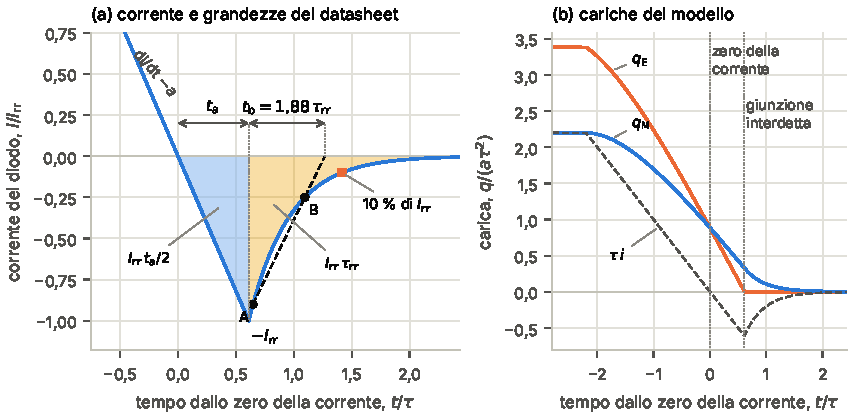
\includegraphics[width=\textwidth]{figures/fig_waveform_it.pdf}
\caption{Spegnimento del modello su una rampa di corrente ($\rho = \lmFigRho$, $\IF/(a\tau) = \lmFigLam$). (a) Corrente e grandezze del datasheet: il triangolo di carica $\Irr\ta/2$, la tail di carica $\Irr\taurr$, la retta per i punti A (\SI{90}{\percent}) e B (\SI{25}{\percent}) che definisce $\tb$, e il punto al \SI{10}{\percent}. (b) Le due cariche del modello e, tratteggiata, $\tau i$: la middle charge $\qM$ segue la corrente con un ritardo, l'edge charge $\qE$ raggiunge lo zero dopo la corrente, e in quell'istante la giunzione entra in interdizione.}
\label{fig:waveform}
\end{figure}

\subsection{Forward characteristic}
Per un diodo raddrizzatore il datasheet fornisce la forward voltage a una corrente e un'approssimazione lineare della caratteristica alla massima temperatura,
\begin{equation}
v \approx \VTo + \rT\, i ,
\label{eq:line}
\end{equation}
con la threshold voltage $\VTo$ e la slope resistance $\rT$. La retta interseca la caratteristica reale a due correnti, che il datasheet dichiara o che sono implicite nel campo di validità della retta. Per un fast diode il datasheet fornisce la forward voltage alla corrente nominale e una curva a due temperature.

\subsection{Blocking state}
Il datasheet fornisce la reverse current $\Irrm$ alla repetitive peak reverse voltage $\Vrrm$ e alla massima temperatura, come valore massimo. Una junction capacitance è data per i diodi piccoli e veloci, a bassa reverse voltage; per i grandi diodi raddrizzatori di solito non è data.

%=====================================================================
\section{Il modello}
\label{sec:model}
\subsection{Equazioni}
Il modello descrive i portatori di carica immagazzinati nella regione centrale debolmente drogata del diodo (la base) con due cariche (Fig.~\ref{fig:model}a). La \emph{middle charge} $\qM$ è la stored charge nella base. La \emph{edge charge} $\qE$ rappresenta la concentrazione dei portatori ai bordi della base, accanto alla giunzione, ed è legata alla junction voltage. I portatori diffondono dal bordo verso il centro, e questa diffusione è la corrente del diodo:
\begin{align}
\idif &= \frac{\qE - \qM}{\TM} , \label{eq:idif}\\
\frac{\diff \qM}{\diff t} &= \idif - \frac{\qM}{\tau} , \label{eq:qm}\\
\qE &= (\tau+\TM)\,\IS\,\bigl(e^{\vj/(n\VT)} - 1\bigr) . \label{eq:qe}
\end{align}
L'equazione \eqref{eq:qm} è il bilancio della middle charge: la diffusion current la alimenta e la ricombinazione la rimuove con il lifetime $\tau$. L'equazione \eqref{eq:idif} dice che la corrente è sostenuta dalla differenza tra le due cariche e che $\TM$ è il tempo che i portatori impiegano a diffondere nella base. L'equazione \eqref{eq:qe} è la junction law. Il diodo completo aggiunge la junction capacitance, una leakage resistance e una resistenza serie:
\begin{equation}
i = \idif + \Cj(\vj)\,\frac{\diff \vj}{\diff t} + \frac{\vj}{\Rr} , \qquad v = \vj + \RS\, i .
\label{eq:terminal}
\end{equation}
Il modello ha un solo stato per la stored charge, $\qM$, perché $\qE$ è una funzione algebrica della junction voltage. Le equazioni sono la descrizione a lumped charge di Linvill \cite{linvill1958} applicata alla base di un diodo di potenza \cite{lauritzen1991}; l'Appendice~\ref{app:lumped} mostra da dove vengono e che cosa è $\TM$ in termini di larghezza della base.

In \eqref{eq:qe} il fattore davanti alla parentesi è scritto in modo che $\IS$ sia la saturation current della caratteristica statica, come in \cite{mathworks}. Alcune implementazioni, tra cui il componente di libreria \texttt{diode\_rr}, scrivono $\qE = \tau\,\IS^{*}\,(e^{\vj/(n\VT)}-1)$. Le due forme sono lo stesso modello con
\begin{equation}
\IS^{*} = \IS\,\frac{\tau+\TM}{\tau} .
\label{eq:isstar}
\end{equation}

\begin{figure}[htb]
\centering
\begin{circuitikz}[scale=0.9, transform shape]
\ctikzset{bipoles/length=1.0cm}
% (a) il modello
\node[anchor=west] at (-0.6,2.6) {(a)};
\draw (0,0) node[left]{A} to[short, o-] (0.3,0) to[R, l=$\RS$] (2.3,0) coordinate (J);
\draw (J) -- (2.3,1.5) to[american controlled current source, l={$\idif$}] (5.3,1.5) -- (5.3,0) coordinate (K);
\draw (J) to[C, l=$\Cj(\vj)$, *-*] (K);
\draw (J) -- (2.3,-1.5) to[R, l=$\Rr$] (5.3,-1.5) -- (K);
\draw (K) to[short, -o] (6.2,0) node[right]{K};
\draw[-{Latex[length=2mm]}] (0.4,0.42) -- (0.95,0.42) node[midway, above]{$i$};
\node at (2.55,-2.0) {$+$}; \node at (3.8,-2.0) {$\vj$}; \node at (5.05,-2.0) {$-$};
% (b) la commutation cell
\begin{scope}[xshift=8.8cm, yshift=-1.6cm]
\node[anchor=west] at (-0.9,4.2) {(b)};
\draw (0,0) to[american voltage source, invert, l=$\VR$] (0,3.2) to[closing switch, l={$t=0$}] (1.7,3.2) to[L, l=$L$] (3.4,3.2) -- (6.4,3.2);
\draw (3.4,0) to[D*, l=D, *-*] (3.4,3.2);
\draw (4.9,3.2) to[R, l=$\Rsn$, *-] (4.9,1.6) to[C, l=$\Csn$, -*] (4.9,0);
\draw (6.4,3.2) to[american current source, l=$\IF$] (6.4,0);
\draw (0,0) -- (6.4,0);
\draw[-{Latex[length=2mm]}] (3.05,0.35) -- (3.05,0.95) node[midway, left]{$i$};
\end{scope}
\end{circuitikz}
\caption{(a) Circuito equivalente del modello: la diffusion current $\idif = (\qE-\qM)/\TM$, con $\qM$ da \eqref{eq:qm} e $\qE$ da \eqref{eq:qe}, in parallelo alla junction capacitance e alla leakage resistance, e in serie a $\RS$. (b) Commutation cell: il diodo conduce la corrente $\IF$ del carico; a $t=0$ l'interruttore applica la tensione $\VR$ in inverso attraverso l'induttanza $L$, e la corrente del diodo scende con il di/dt $a = \VR/L$. Uno snubber RC può essere posto in parallelo al diodo.}
\label{fig:model}
\end{figure}

\subsection{Caratteristica statica}
In regime stazionario $\diff\qM/\diff t = 0$, quindi \eqref{eq:idif} e \eqref{eq:qm} danno
\begin{equation}
\qM = \tau\, i , \qquad \qE = (\tau+\TM)\, i , \qquad i = \IS\,\bigl(e^{\vj/(n\VT)}-1\bigr) .
\label{eq:static}
\end{equation}
A riposo il modello è l'ordinaria equazione del diodo con una resistenza serie, e la base contiene la carica $\tau\,i$. I parametri $\IS$, $n$ e $\RS$ danno forma alla forward characteristic e non hanno alcun ruolo nel recovery, purché la forward voltage sia piccola rispetto alle tensioni del circuito.

\subsection{Due regimi e due costanti di tempo}
\label{sec:regimes}
Il diodo lavora in uno di due regimi.

\emph{Giunzione in conduzione} ($\qE > 0$). La junction voltage è una forward voltage dell'ordine di un volt, qualunque sia il segno della corrente. Il circuito impone la corrente, e le cariche la seguono: con $\idif = i$,
\begin{equation}
\frac{\diff \qM}{\diff t} = i - \frac{\qM}{\tau} , \qquad \qE = \qM + \TM\, i .
\label{eq:conducting}
\end{equation}
La prima relazione è la classica equazione del controllo di carica con la costante di tempo $\tau$. La seconda dice che l'edge charge è la middle charge più una parte proporzionale alla corrente. In questo regime può scorrere una reverse current: basta che sia $\qM > \TM\,|i|$.

\emph{Giunzione interdetta} ($\qE = 0$). L'edge charge non può scendere sotto zero: in \eqref{eq:qe} una reverse voltage porta la parentesi a $-1$ e $\qE$ a $-(\tau+\TM)\IS$, che è nulla sulla scala della stored charge. Con $\qE = 0$,
\begin{equation}
\idif = -\frac{\qM}{\TM} , \qquad \frac{\diff\qM}{\diff t} = -\qM\Bigl(\frac1\TM + \frac1\tau\Bigr) = -\frac{\qM}{\taurr} , \qquad \taurr = \frac{\tau\,\TM}{\tau+\TM} .
\label{eq:blocked}
\end{equation}
Il diodo è ora un generatore di corrente che decade con la costante di tempo $\taurr$, qualunque cosa faccia il circuito; il circuito impone la tensione. La carica rimasta nella base esce per diffusione verso i bordi (la reverse current) e per ricombinazione, e le due velocità si sommano. La tail time constant è sempre più breve sia di $\tau$ sia di $\TM$. Il rapporto
\begin{equation}
\rho = \frac{\taurr}{\tau} = \frac{\TM}{\tau+\TM}
\label{eq:rho}
\end{equation}
è usato nel seguito come parametro di forma del modello, con $0 < \rho < 1$.

Vista dalla corrente, l'edge charge della giunzione in conduzione è una copia filtrata della corrente. Da \eqref{eq:conducting}, nel dominio di Laplace,
\begin{equation}
\frac{\qE(s)}{i(s)} = (\tau+\TM)\,\frac{1+s\,\taurr}{1+s\,\tau} .
\label{eq:filter}
\end{equation}
È una rete ritardatrice. Per una corrente che varia lentamente sulla scala di $\tau$ è un puro ritardo di $\tau-\taurr$: l'edge charge è $(\tau+\TM)$ volte la corrente di $\tau-\taurr$ prima. La giunzione entra in interdizione quando $\qE$ attraversa lo zero, quindi su una rampa lenta lo fa $\tau-\taurr$ dopo lo zero della corrente, quando la reverse current è cresciuta fino a $a\,(\tau-\taurr)$. È l'intero reverse recovery del modello in una riga; la Sezione~\ref{sec:ramp} lo rende esatto.

\subsection{Parametri}
\begin{table}[htb]
\centering\small
\caption{Parametri del modello e dati del datasheet che li fissano.}
\label{tab:params}
\begin{tabular}{@{}llp{6.4cm}c@{}}
\toprule
Parametro & Ruolo & Dati del datasheet & Sezione \\
\midrule
$\tau$, $\TM$ & reverse recovery & due tra $\Irr$, $\Qrr$, $\trr$ a di/dt e forward current dichiarati & \ref{sec:inverse} \\
$\IS$, $n$, $\RS$ & forward characteristic & $\VTo$ e $\rT$, oppure punti della forward curve & \ref{sec:forward} \\
$\Rr$ & leakage nel blocking state & reverse current a una reverse voltage & \ref{sec:blocking} \\
$\Cjo$, $V_\mathrm{j}$, $m$ & junction capacitance & capacità a una reverse voltage, oppure una stima & \ref{sec:blocking} \\
\bottomrule
\end{tabular}
\end{table}
I quattro gruppi della Tabella~\ref{tab:params} sono indipendenti: ciascuno si può convertire senza gli altri. I parametri del recovery sono l'oggetto delle prossime tre sezioni.

%=====================================================================
\section{Spegnimento su una rampa di corrente}
\label{sec:ramp}
\subsection{Ipotesi}
Il diodo è in regime stazionario con la forward current $\IF$. Da $t = 0$ il circuito forza la corrente a scendere con la velocità costante $a$:
\begin{equation}
i(t) = \IF - a\,t .
\label{eq:ramp}
\end{equation}
Nella commutation cell della Fig.~\ref{fig:model}b il di/dt è $a = \VR/L$. Il circuito impone la rampa finché la giunzione conduce, perché la junction voltage è piccola rispetto a $\VR$. La junction capacitance e il leakage sono trascurati in questa sezione; la Sezione~\ref{sec:cell} mostra il loro effetto sui due esempi.

\subsection{Cariche durante la rampa}
Con \eqref{eq:ramp} e il valore iniziale $\qM(0) = \tau\IF$, la soluzione di \eqref{eq:conducting} è
\begin{align}
\qM(t) &= \tau\,(\IF - a\,t) + a\,\tau^2\,\bigl(1 - e^{-t/\tau}\bigr) , \label{eq:qmramp}\\
\qE(t) &= (\tau+\TM)\,(\IF - a\,t) + a\,\tau^2\,\bigl(1 - e^{-t/\tau}\bigr) . \label{eq:qeramp}
\end{align}
Il primo termine di \eqref{eq:qmramp} è la carica che il diodo avrebbe se seguisse la corrente senza ritardo. Il secondo termine è il ritardo: carica ancora presente nella base perché la ricombinazione richiede tempo. Allo zero della corrente, $t_0 = \IF/a$, il primo termine si annulla e le due cariche sono uguali:
\begin{equation}
\qM(t_0) = a\,\tau^2\,\bigl(1 - e^{-\IF/(a\tau)}\bigr) .
\label{eq:qzero}
\end{equation}
La carica presente allo zero della corrente non è la carica statica $\tau\IF$. Su una rampa che dura diversi lifetime è $a\,\tau^2$, qualunque sia la forward current: la carica presente all'inizio si è ricombinata lungo il percorso, e ciò che resta è quanto hanno alimentato gli ultimi lifetime della rampa. La Figura~\ref{fig:waveform}b mostra le due cariche.

\subsection{Peak reverse current}
La giunzione entra in interdizione all'istante $\Tone$ in cui $\qE$ raggiunge lo zero. La corrente in quell'istante è il picco, $i(\Tone) = -\Irr$, quindi $\Tone = (\IF+\Irr)/a$. L'equazione \eqref{eq:qeramp} con $\qE(\Tone) = 0$, e con $\tau^2/(\tau+\TM) = \tau - \taurr$, dà
\begin{equation}
\Irr = a\,(\tau-\taurr)\,\bigl(1 - e^{-\Tone/\tau}\bigr) , \qquad \Tone = \frac{\IF+\Irr}{a} .
\label{eq:peak}
\end{equation}
È un'equazione implicita in $\Irr$, perché $\Tone$ la contiene. Il tempo dallo zero della corrente al picco è $\ta = \Irr/a$. Fino al picco la tensione del diodo è ancora una piccola forward voltage, benché la corrente sia già invertita.

\subsection{Tail e recovered charge}
Dopo $\Tone$ la giunzione è interdetta e vale \eqref{eq:blocked}, con $\qM(\Tone) = \TM\Irr$:
\begin{equation}
i(t) = -\Irr\,e^{-(t-\Tone)/\taurr} , \qquad t \geq \Tone .
\label{eq:tail}
\end{equation}
La reverse current è un triangolo di base $\ta$ seguito da un esponenziale, con uno spigolo al picco. Il suo integrale è la recovered charge
\begin{equation}
\Qrr = \frac{\Irr\,\ta}{2} + \Irr\,\taurr = \frac{\Irr^2}{2a} + \Irr\,\taurr .
\label{eq:qrr}
\end{equation}
L'equazione \eqref{eq:qrr} vale per qualunque durata della rampa: usa solo la forma d'onda.

\subsection{Forma normalizzata e soluzione in forma chiusa}
\label{sec:norm}
Con le grandezze normalizzate
\begin{equation}
y = \frac{\Irr}{a\,\tau} , \qquad \lambda = \frac{\IF}{a\,\tau} , \qquad \rho = \frac{\taurr}{\tau} ,
\label{eq:normdef}
\end{equation}
le equazioni \eqref{eq:peak} e \eqref{eq:qrr} diventano
\begin{equation}
y = (1-\rho)\,\bigl(1 - e^{-(\lambda+y)}\bigr) , \qquad \frac{\Qrr}{a\,\tau^2} = \frac{y^2}{2} + \rho\,y .
\label{eq:norm}
\end{equation}
Il recovery normalizzato dipende da due soli numeri: il parametro di forma $\rho$, e $\lambda$, che è il tempo impiegato dalla rampa per raggiungere lo zero della corrente contato in lifetime. La prima delle \eqref{eq:norm} ha la soluzione
\begin{equation}
y = (1-\rho) + W_0\!\left(-(1-\rho)\,e^{-(\lambda+1-\rho)}\right) ,
\label{eq:lambert}
\end{equation}
dove $W_0$ è il ramo principale della funzione di Lambert, l'inversa di $w \mapsto w\,e^{w}$ (Appendice~\ref{app:lambert}). Il termine di Lambert è negativo: è ciò che la durata finita della rampa toglie al valore per rampa lunga $1-\rho$. La Figura~\ref{fig:map} mostra il risultato.

\begin{figure}[htb]
\centering
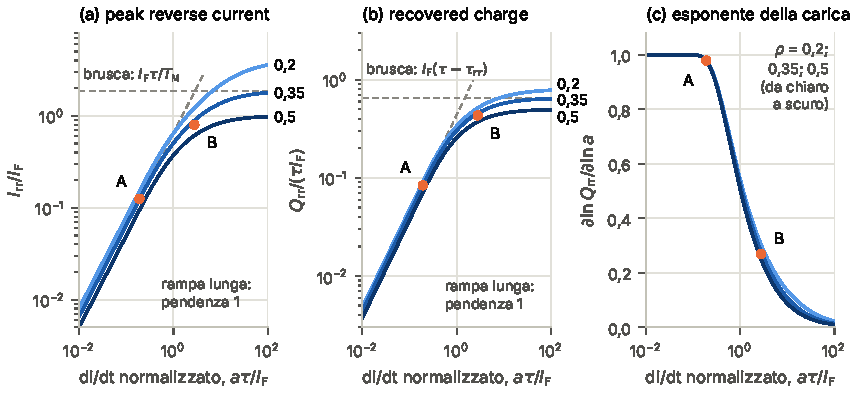
\includegraphics[width=\textwidth]{figures/fig_map_it.pdf}
\caption{Recovery del modello in funzione del di/dt normalizzato $a\tau/\IF = 1/\lambda$, per tre valori di $\rho$. (a) Peak reverse current e (b) recovered charge, con i due asintoti della curva centrale: la rampa lunga \eqref{eq:long}, con pendenza uno, e la commutazione brusca \eqref{eq:abrupt}, una costante. (c) Esponente locale della carica rispetto al di/dt, \eqref{eq:exponents}. I punti A e B sono i due esempi svolti della Sez.~\ref{sec:examples} nelle loro condizioni di datasheet.}
\label{fig:map}
\end{figure}

\subsection{Rampa lunga e commutazione brusca}
\label{sec:limitsramp}
\emph{Rampa lunga} ($\lambda \to \infty$). L'esponenziale di \eqref{eq:peak} si annulla:
\begin{equation}
\Irr = a\,(\tau - \taurr) = \frac{a\,\tau^2}{\tau+\TM} , \qquad \ta = \tau - \taurr , \qquad \Qrr = \frac{a}{2}\,\bigl(\tau^2 - \taurr^2\bigr) .
\label{eq:long}
\end{equation}
Picco e carica sono proporzionali al di/dt e non dipendono dalla forward current. Il tempo al picco è una costante del diodo: è il ritardo $\tau - \taurr$ di \eqref{eq:filter}.

Il fattore $1 - e^{-x}$ di \eqref{eq:peak}, con $x = \Tone/\tau$, dice quanto deve essere lunga una rampa. La Tabella~\ref{tab:long} riporta quanto manca ai valori per rampa lunga. Ai fini di una conversione una rampa è lunga quando dura cinque lifetime dalla forward current al picco; con tre lifetime le formule per rampa lunga sbagliano del \SI{\lmFDefThree}{\percent} sul picco e fino al \SI{\lmQDefHiThree}{\percent} sulla carica.

\begin{table}[htb]
\centering\small
\caption{Corrente di picco e carica del modello su una rampa di durata finita, rispetto ai valori per rampa lunga \eqref{eq:long}. L'intervallo della carica è per $\rho$ da 0,5 a 0,1.}
\label{tab:long}
\begin{tabular}{@{}lcccc@{}}
\toprule
Durata della rampa, $x = \Tone/\tau$ & 2 & 3 & 4 & 5 \\
\midrule
$\Irr$ inferiore al valore per rampa lunga del & \SI{\lmFDefTwo}{\percent} & \SI{\lmFDefThree}{\percent} & \SI{\lmFDefFour}{\percent} & \SI{\lmFDefFive}{\percent} \\
$\Qrr$ inferiore al valore per rampa lunga del & \SIrange{\lmQDefLoTwo}{\lmQDefHiTwo}{\percent} & \SIrange{\lmQDefLoThree}{\lmQDefHiThree}{\percent} & \SIrange{\lmQDefLoFour}{\lmQDefHiFour}{\percent} & \SIrange{\lmQDefLoFive}{\lmQDefHiFive}{\percent} \\
\bottomrule
\end{tabular}
\end{table}

\emph{Commutazione brusca} ($\lambda \to 0$). La rampa è così rapida che nulla si ricombina prima che la giunzione entri in interdizione. La middle charge è ancora $\tau\IF$ quando l'edge charge è portata a zero, e \eqref{eq:blocked} dà
\begin{equation}
\Irr \to \IF\,\frac{\tau}{\TM} , \qquad \Qrr \to \IF\,(\tau - \taurr) = \IF\,\frac{\tau^2}{\tau+\TM} .
\label{eq:abrupt}
\end{equation}
Picco e carica sono proporzionali alla forward current e non dipendono più dal di/dt. Sono i valori più grandi che il modello può dare per una data forward current.

\subsection{Bilancio della carica}
Della carica presente allo zero della corrente, \eqref{eq:qzero}, solo una parte esce dai terminali. Il resto si ricombina durante il recovery. Su una rampa lunga, da \eqref{eq:long},
\begin{equation}
\frac{\Qrr}{\qM(t_0)} = \frac{1-\rho^2}{2} .
\label{eq:fraction}
\end{equation}
Viene recuperata meno della metà della carica presente allo zero della corrente: il \SI{\lmQfracRhoLo}{\percent} per $\rho = 0,2$, il \SI{\lmQfracRhoMid}{\percent} per $\rho = 0,35$, il \SI{\lmQfracRhoHi}{\percent} per $\rho = 0,5$. In una commutazione brusca la parte recuperata della carica statica $\tau\IF$ è $1-\rho$, da \eqref{eq:abrupt}. La recovered charge di un datasheet non è quindi mai la stored charge del diodo, e il lifetime non si può leggere come $\Qrr/\IF$ (Sez.~\ref{sec:others}).

\subsection{Dipendenza dal di/dt e dalla forward current}
\label{sec:exponents}
Finché la giunzione conduce, le equazioni \eqref{eq:conducting} sono lineari, e la condizione di interdizione $\qE = 0$ non cambia se la corrente e le cariche sono tutte moltiplicate per lo stesso fattore. Quindi se il di/dt e la forward current sono entrambi moltiplicati per $k$, l'intera forma d'onda è moltiplicata per $k$: $\Irr$ e $\Qrr$ sono funzioni omogenee di grado uno della coppia $(a, \IF)$, come mostrano \eqref{eq:normdef} e \eqref{eq:norm}. Per il teorema di Eulero sulle funzioni omogenee
\begin{equation}
\frac{\partial \ln \Irr}{\partial \ln a} + \frac{\partial \ln \Irr}{\partial \ln \IF} = 1 , \qquad
\frac{\partial \ln \Qrr}{\partial \ln a} + \frac{\partial \ln \Qrr}{\partial \ln \IF} = 1 .
\label{eq:euler}
\end{equation}
In un diagramma bilogaritmico la pendenza di una curva in funzione di $a$ e la pendenza della curva in funzione di $\IF$ sommano a uno, in ogni punto. Gli esponenti rispetto al di/dt discendono da \eqref{eq:norm} (Appendice~\ref{app:exponents}):
\begin{equation}
\frac{\partial \ln \Irr}{\partial \ln a} = 1 - \frac{\lambda\,(1-\rho-y)}{y\,(\rho+y)} , \qquad
\frac{\partial \ln \Qrr}{\partial \ln a} = 1 - \frac{\lambda\,(1-\rho-y)}{y^2/2+\rho\,y} .
\label{eq:exponents}
\end{equation}
Su una rampa lunga $y = 1-\rho$ ed entrambi gli esponenti valgono uno: il recovery è proporzionale al di/dt e insensibile alla forward current. In una commutazione brusca entrambi valgono zero e il recovery è proporzionale alla forward current. La Figura~\ref{fig:map}c mostra il passaggio dall'uno all'altro, che richiede circa due decadi di di/dt attorno ad $a\tau = \IF$.

%=====================================================================
\section{Dal modello alle grandezze del datasheet}
\label{sec:direct}
\subsection{Recovery time e softness}
\label{sec:trr}
Con la tail esponenziale \eqref{eq:tail}, ogni convenzione per la fine del recovery dà un fall time proporzionale alla tail time constant:
\begin{equation}
\tb = \kappa\,\taurr , \qquad \trr = \ta + \kappa\,\taurr .
\label{eq:trr}
\end{equation}
Per una retta per i punti alle frazioni $p_\mathrm{A}$ e $p_\mathrm{B}$ del picco,
\begin{equation}
\kappa = \ln\frac{1}{p_\mathrm{A}} + \frac{p_\mathrm{A}}{p_\mathrm{A}-p_\mathrm{B}}\,\ln\frac{p_\mathrm{A}}{p_\mathrm{B}} ,
\label{eq:kappaline}
\end{equation}
e per l'istante in cui la corrente è scesa alla frazione $p$ del picco, $\kappa = \ln(1/p)$. La Tabella~\ref{tab:kappa} riporta i valori. Tra le convenzioni il fall time della stessa forma d'onda differisce fino a \num{\lmKSpread} tail time constant, quindi un recovery time non si può convertire senza la sua convenzione.

\begin{table}[htb]
\centering\small
\caption{Convenzioni per la fine del recovery e fall time di una tail esponenziale, $\tb = \kappa\,\taurr$.}
\label{tab:kappa}
\begin{tabular}{@{}lcl@{}}
\toprule
Convenzione & $\kappa$ & Usata in \\
\midrule
retta per il \SI{90}{\percent} e il \SI{25}{\percent} del picco, prolungata fino a zero & \lmKLine & \cite{iec60747}, 3.5.2 Nota~5; \cite{an6481}, Sez.~2.1 \\
corrente scesa al \SI{25}{\percent} del picco & \lmKQuarter & \cite{an5028} ($k$ di solito \num{0.25}) \\
corrente scesa al \SI{10}{\percent} del picco & \lmKTen & \cite{mathworks}, \cite{plecs} \\
triangolo con la stessa carica della tail & 2 & questa nota, \eqref{eq:soft} \\
\bottomrule
\end{tabular}
\end{table}

Questa nota misura la softness con il rapporto tra la carica della tail e la carica del triangolo,
\begin{equation}
s = \frac{\Irr\,\taurr}{\Irr\,\ta/2} = \frac{2\,\taurr}{\ta} .
\label{eq:soft}
\end{equation}
È il rapporto $\tb/\ta$ per il triangolo di uguale carica ($\kappa = 2$); il rapporto $\tb/\ta$ della convenzione della retta è \num{\lmKLineHalf}\,$s$. Da \eqref{eq:peak}, $\ta = (\tau-\taurr)\,(1-e^{-x})$, quindi
\begin{equation}
s = \frac{2\,\TM}{\tau}\,\frac{1}{1-e^{-x}} \quad\longrightarrow\quad s = \frac{2\,\TM}{\tau} \quad \text{su una rampa lunga.}
\label{eq:softlong}
\end{equation}
Su una rampa lunga la softness del modello è una costante del diodo: il doppio del rapporto tra i suoi due parametri. Non dipende dal di/dt, dalla forward current o dalla tensione. Su una rampa corta la softness è maggiore, perché il triangolo si accorcia e la tail time constant no. La documentazione \cite{mathworks} usa il \emph{stretch factor} $\trr\,a/\Irr$ con la convenzione del \SI{10}{\percent}, che vale $1 + (\ln 10/2)\,s$; il suo valore tipico di 3 corrisponde a $s = \lmSofStretchThree$.

\subsection{Recovered charge}
L'equazione \eqref{eq:qrr} è l'integrale dell'intera reverse current. Se l'integrale termina dove la corrente è scesa alla frazione $p$ del picco, come nella norma con $p = \SI{\lmPEndPct}{\percent}$, viene tagliata la frazione $p$ della carica della tail:
\begin{equation}
Q_\mathrm{r} = \frac{\Irr\,\ta}{2} + (1-p)\,\Irr\,\taurr .
\label{eq:qrp}
\end{equation}
L'integrale dura allora $\ln(1/p) = \lmTEndTaus$ tail time constant. La differenza rispetto a \eqref{eq:qrr} è inferiore alla tolleranza di qualunque valore di datasheet; è usata nella Sez.~\ref{sec:cell} per confrontare una simulazione con la forma chiusa ad armi pari. Una seconda differenza è la carica della junction capacitance, che un valore misurato comprende e \eqref{eq:qrr} no (Sez.~\ref{sec:blocking}).

La stima $\Qrr \approx \Irr\,\trr/2$ è esatta con la convenzione di uguale carica. Con la convenzione della retta perde il \SI{\lmKLineLossPct}{\percent} della carica della tail, e con la convenzione del \SI{10}{\percent} vi aggiunge il \SI{\lmKTenGainPct}{\percent}.

\subsection{Tensione di picco ed energia in una commutazione induttiva}
\label{sec:energy}
Nella cella della Fig.~\ref{fig:model}b senza snubber e senza capacità, la tensione del diodo resta vicina a zero fino al picco della reverse current. Nella tail il diodo impone all'induttanza la corrente \eqref{eq:tail}, e la sua reverse voltage è
\begin{equation}
v_\mathrm{R}(t) = \VR + \frac{L\,\Irr}{\taurr}\,e^{-(t-\Tone)/\taurr} .
\end{equation}
Il picco si ha nell'istante di interdizione. Con $L = \VR/a$,
\begin{equation}
\Vrm = \VR + \frac{L\,\Irr}{\taurr} = \VR\,\Bigl(1 + \frac{\ta}{\taurr}\Bigr) = \VR\,\Bigl(1 + \frac{2}{s}\Bigr) .
\label{eq:vrm}
\end{equation}
La tensione di picco dipende solo dalla softness: un diodo con $s = 1$ triplica la tensione applicata, uno con $s = 4$ ne aggiunge la metà. L'energia dissipata nel diodo durante la tail è
\begin{equation}
E = \int v_\mathrm{R}\,|i|\,\diff t = \VR\,\Irr\,\taurr + \frac{L\,\Irr^2}{2} = \VR\,\Qrr .
\label{eq:erec}
\end{equation}
La prima forma è in \cite{mathworks}; la seconda segue con $L = \VR/a$ e \eqref{eq:qrr}. Contiene l'energia che l'induttanza possiede al picco.

Nel modello la tensione passa a gradino da zero a $\Vrm$ nell'istante di interdizione. Un circuito reale ha capacità in parallelo al diodo, che arrotonda il gradino e può abbassare il picco; uno snubber lo fa di proposito. Con uno snubber RC in parallelo al diodo il bilancio dell'energia dallo zero della corrente alla fine del transitorio è
\begin{equation}
E_\mathrm{D} + E_\mathrm{R} = \VR\,\Qrr + \frac{\Csn\,\VR^2}{2} ,
\label{eq:ebal}
\end{equation}
dove $E_\mathrm{D}$ è l'energia dissipata nel diodo ed $E_\mathrm{R}$ l'energia dissipata nel resistore dello snubber. La sorgente eroga $\VR$ per la carica del diodo e del condensatore dello snubber, e il condensatore trattiene $\Csn\VR^2/2$. La somma non dipende dal resistore dello snubber: lo snubber sposta una parte di $\VR\,\Qrr$ dal diodo al resistore e aggiunge la perdita di carica del suo condensatore.

\subsection{Altri circuiti di prova}
\label{sec:othertests}
\emph{Commutazione resistiva.} I diodi piccoli e veloci sono spesso provati con un gradino: la forward current $\IF$ è invertita bruscamente e il circuito limita la reverse current a $\IR$. Finché la giunzione conduce, la reverse current resta a $\IR$; è la fase di storage. L'equazione \eqref{eq:conducting} con $i = -\IR$ dà $\qM(t) = -\tau\IR + \tau\,(\IF+\IR)\,e^{-t/\tau}$, e $\qE = \qM - \TM\IR$ raggiunge lo zero allo storage time
\begin{equation}
\ts = \tau\,\ln\!\left[\Bigl(1+\frac{\IF}{\IR}\Bigr)\,\frac{\tau}{\tau+\TM}\right] \qquad \text{se} \quad \frac{\IF}{\IR} > \frac{\TM}{\tau} .
\label{eq:ts}
\end{equation}
Dopo lo storage time la corrente decade da $\IR$ con la costante di tempo $\taurr$. Se $\IF/\IR \leq \TM/\tau$ non c'è fase di storage: la giunzione entra subito in interdizione, la reverse current parte da $\IF\,\tau/\TM$, che è il limite brusco \eqref{eq:abrupt}, e decade da lì. Con $\TM \to 0$ l'equazione \eqref{eq:ts} diventa $\ts = \tau\ln(1+\IF/\IR)$, lo storage time del modello a controllo di carica con una sola carica.

\emph{Impulso semisinusoidale.} La norma prevede un metodo di misura semisinusoidale e uno rettangolare (\cite{iec60747}, 6.3.5). Per una corrente sinusoidale $\hat I\sin\omega t$ che è durata a lungo sulla scala di $\tau$, \eqref{eq:filter} dà l'edge charge come una sinusoide ritardata della fase $\arctan\omega\tau - \arctan\omega\taurr$. La giunzione entra in interdizione a questa fase dopo lo zero della corrente, quindi
\begin{equation}
\Irr = \hat I\,\sin\bigl(\arctan\omega\tau - \arctan\omega\taurr\bigr) .
\label{eq:sine}
\end{equation}
Per $\omega\tau \ll 1$ questa è $\omega\hat I\,(\tau-\taurr)$: il risultato per rampa lunga \eqref{eq:long} con il di/dt $a = \omega\hat I$ della sinusoide al suo zero.

%=====================================================================
\section{Dal datasheet al modello}
\label{sec:inverse}
\subsection{Dalla corrente di picco e dalla carica}
\label{sec:invpq}
Il datasheet fornisce $\Irr$ e $\Qrr$ a un di/dt $a$ e a una forward current $\IF$. La conversione ha quattro passi.
\begin{enumerate}
\item Tempo al picco: $\ta = \Irr/a$.
\item Tail time constant, da \eqref{eq:qrr}:
\begin{equation}
\taurr = \frac{\Qrr}{\Irr} - \frac{\Irr}{2a} .
\label{eq:taurr}
\end{equation}
Questo passo è esatto per qualunque rampa; la stessa relazione è l'Eq.~(2) di \cite{an6481}. Richiede $\Qrr > \Irr^2/(2a)$: la carica deve essere maggiore del triangolo. Una coppia di dati che viola la condizione non ha tail e non può essere rappresentata dal modello.
\item Lifetime, da \eqref{eq:peak} scritta come
\begin{equation}
\tau = \taurr + \frac{\ta}{1 - e^{-\Tone/\tau}} , \qquad \Tone = \frac{\IF+\Irr}{a} .
\label{eq:iter}
\end{equation}
L'equazione \eqref{eq:iter} si usa come iterazione: il secondo membro è valutato con il valore corrente di $\tau$, partendo da $\tau = \taurr + \ta$. L'iterazione converge per qualunque dato, all'unica soluzione, e a ogni passo l'errore si riduce di un fattore minore di $\Irr/(\IF+\Irr)$ (Appendice~\ref{app:contraction}).
\item Transit time, dalla definizione di $\taurr$:
\begin{equation}
\TM = \frac{\tau\,\taurr}{\tau - \taurr} .
\label{eq:tm}
\end{equation}
\end{enumerate}
Su una rampa lunga l'esponenziale di \eqref{eq:iter} è nullo e il valore di partenza è già il risultato:
\begin{equation}
\tau = \taurr + \ta = \frac{\Qrr}{\Irr} + \frac{\Irr}{2a} , \qquad \TM = \frac{\tau\,\taurr}{\ta} .
\label{eq:longinv}
\end{equation}
È la forma chiusa che si trova nelle note sul modello; non contiene la forward current.

\subsection{Quando basta la forma chiusa}
\label{sec:valid}
La forma chiusa \eqref{eq:longinv} è esatta per $x = \Tone/\tau \to \infty$. Se un punto del datasheet sia su una rampa lunga si vede dai soli dati, perché $x$ discende dal rapporto $\Irr/\IF$ e dalla softness $s = 2\taurr/\ta$:
\begin{equation}
x = \frac{1 + \IF/\Irr}{s/2 + 1/(1-e^{-x})} \;\approx\; \frac{1 + \IF/\Irr}{1 + s/2} .
\label{eq:xdata}
\end{equation}
Un set di parametri ottenuto con la forma chiusa da un punto che non è su una rampa lunga non è il diodo del datasheet: riportato sulla rampa di prova restituisce un picco più basso e una carica più bassa. La Figura~\ref{fig:inversion} mostra questo errore e la Tabella~\ref{tab:valid} ne dà i limiti. Quando la peak reverse current del datasheet è sotto un decimo della forward current, il set della forma chiusa restituisce il picco e la carica entro il \SI{\lmTenthErrTwo}{\percent} per una softness fino a 2 ed entro il \SI{\lmTenthErrFour}{\percent} per una softness di 4. Per un fast diode provato con una peak reverse current vicina alla forward current sbaglia di decine di punti percentuali, e va usata la \eqref{eq:iter}. L'iterazione non costa nulla, quindi la regola semplice è iterare sempre.

\begin{table}[htb]
\centering\small
\caption{Massimo rapporto $\Irr/\IF$ del punto del datasheet per cui il set della forma chiusa \eqref{eq:longinv} restituisce la corrente di picco del datasheet entro l'errore indicato.}
\label{tab:valid}
\begin{tabular}{@{}lcccc@{}}
\toprule
Softness del punto del datasheet, $s = 2\taurr/\ta$ & 0,5 & 1 & 2 & 4 \\
\midrule
$\Irr$ restituita entro l'\SI{1}{\percent} per $\Irr/\IF$ sotto & \lmRatioOneHalf & \lmRatioOneOne & \lmRatioOneTwo & \lmRatioOneFour \\
$\Irr$ restituita entro il \SI{5}{\percent} per $\Irr/\IF$ sotto & \lmRatioFiveHalf & \lmRatioFiveOne & \lmRatioFiveTwo & \lmRatioFiveFour \\
\bottomrule
\end{tabular}
\end{table}

\begin{figure}[htb]
\centering
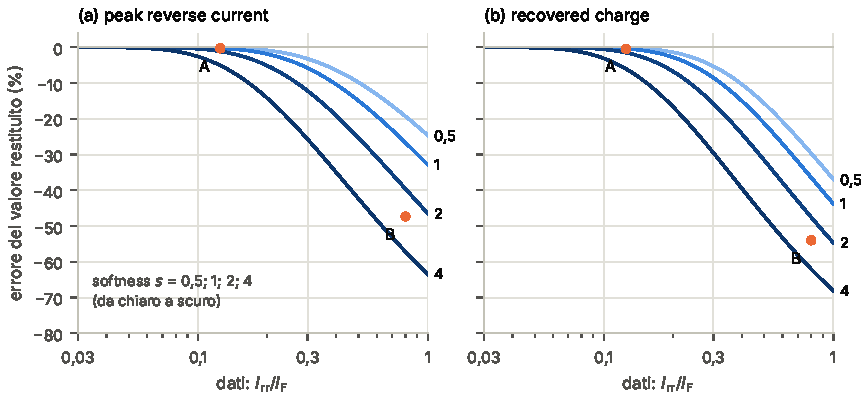
\includegraphics[width=\textwidth]{figures/fig_inversion_it.pdf}
\caption{Errore della forma chiusa per rampa lunga \eqref{eq:longinv}: il set che essa fornisce è riportato sulla rampa di prova e (a) la sua corrente di picco e (b) la sua carica sono confrontate con i dati, in funzione del rapporto $\Irr/\IF$ del punto del datasheet e per quattro valori della softness. A e B sono i due esempi svolti.}
\label{fig:inversion}
\end{figure}

\subsection{Da altre coppie di dati}
\label{sec:pairs}
Il recovery ha due parametri, quindi servono due dati indipendenti in una condizione di prova. Con coppie diverse da $(\Irr, \Qrr)$ cambiano i primi due passi della Sez.~\ref{sec:invpq} e restano gli altri due.

\emph{Corrente di picco e recovery time.} Da \eqref{eq:trr}, con il $\kappa$ della convenzione del datasheet,
\begin{equation}
\taurr = \frac{\trr - \Irr/a}{\kappa} .
\label{eq:fromtrr}
\end{equation}
Richiede $\trr > \Irr/a$.

\emph{Carica e recovery time.} Eliminando $\taurr$ tra \eqref{eq:qrr} e \eqref{eq:trr} si ottiene un'equazione di secondo grado nella corrente di picco, $(1-\kappa/2)\,\Irr^2 - a\,\trr\,\Irr + \kappa\,a\,\Qrr = 0$, con la soluzione
\begin{equation}
\Irr = \frac{a}{2-\kappa}\left[\trr - \sqrt{\trr^2 - \frac{2\,\kappa\,(2-\kappa)\,\Qrr}{a}}\,\right] \quad (\kappa \neq 2) , \qquad \Irr = \frac{2\,\Qrr}{\trr} \quad (\kappa = 2) .
\label{eq:fromqt}
\end{equation}
È la radice con $\Irr < a\,\trr$; esiste quando $\Qrr < a\,\trr^2/2$. Poi \eqref{eq:fromtrr} dà $\taurr$.

\emph{Un solo dato.} Con la sola carica, o il solo recovery time, la forma deve essere ipotizzata. Con una softness ipotizzata $s$, da \eqref{eq:qrr} e \eqref{eq:soft},
\begin{equation}
\Irr = \sqrt{\frac{2\,a\,\Qrr}{1+s}} , \qquad \taurr = \frac{s\,\Irr}{2a} .
\label{eq:fromq}
\end{equation}

\emph{Tre dati.} Quando il datasheet fornisce $\Irr$, $\Qrr$ e $\trr$, i tre sono coerenti con una tail esponenziale se $\Qrr = \Irr\,[\ta/2 + (\trr-\ta)/\kappa]$. Di solito non lo sono esattamente, perché una tail reale non è un esponenziale. La coppia $(\Irr, \Qrr)$ è allora la scelta migliore: il picco e la carica sono ciò che il circuito sente, e non dipendono da una convenzione. Il recovery time serve da verifica.

\subsection{Sensibilità ai dati}
\label{sec:sens}
I valori di datasheet hanno tolleranze, e i due valori di una coppia sono spesso massimi che non appartengono allo stesso dispositivo. Su una rampa lunga le derivate logaritmiche di \eqref{eq:taurr} e \eqref{eq:longinv} sono
\begin{equation}
\begin{aligned}
\frac{\diff\taurr}{\taurr} &= \frac{1+s}{s}\,\frac{\diff\Qrr}{\Qrr} - \frac{2+s}{s}\,\frac{\diff\Irr}{\Irr} + \frac{1}{s}\,\frac{\diff a}{a} , \\
\frac{\diff\tau}{\tau} &= \frac{1+s}{2+s}\,\frac{\diff\Qrr}{\Qrr} - \frac{s}{2+s}\,\frac{\diff\Irr}{\Irr} - \frac{1}{2+s}\,\frac{\diff a}{a} , \\
\frac{\diff\TM}{\TM} &= \frac{\diff\tau}{\tau} + \frac{\diff\taurr}{\taurr} - \frac{\diff\Irr}{\Irr} + \frac{\diff a}{a} .
\end{aligned}
\label{eq:sens}
\end{equation}

\begin{table}[htb]
\centering\small
\caption{Variazione relativa dei parametri per una variazione relativa di un dato dell'uno per cento, su una rampa lunga, da \eqref{eq:sens}.}
\label{tab:sens}
\begin{tabular}{@{}lccccccccc@{}}
\toprule
 & \multicolumn{3}{c}{$s = 0,5$} & \multicolumn{3}{c}{$s = 1$} & \multicolumn{3}{c}{$s = 2$} \\
\cmidrule(lr){2-4}\cmidrule(lr){5-7}\cmidrule(l){8-10}
Dato & $\tau$ & $\taurr$ & $\TM$ & $\tau$ & $\taurr$ & $\TM$ & $\tau$ & $\taurr$ & $\TM$ \\
\midrule
$\Qrr$ & $+\lmSensTauQHalf$ & $+\lmSensTrrQHalf$ & $+\lmSensTmQHalf$ & $+\lmSensTauQOne$ & $+\lmSensTrrQOne$ & $+\lmSensTmQOne$ & $+\lmSensTauQTwo$ & $+\lmSensTrrQTwo$ & $+\lmSensTmQTwo$ \\
$\Irr$ & $-\lmSensTauIHalf$ & $-\lmSensTrrIHalf$ & $-\lmSensTmIHalf$ & $-\lmSensTauIOne$ & $-\lmSensTrrIOne$ & $-\lmSensTmIOne$ & $-\lmSensTauITwo$ & $-\lmSensTrrITwo$ & $-\lmSensTmITwo$ \\
$a$ & $-\lmSensTauAHalf$ & $+\lmSensTrrAHalf$ & $+\lmSensTmAHalf$ & $-\lmSensTauAOne$ & $+\lmSensTrrAOne$ & $+\lmSensTmAOne$ & $-\lmSensTauATwo$ & $+\lmSensTrrATwo$ & $+\lmSensTmATwo$ \\
\bottomrule
\end{tabular}
\end{table}

La Tabella~\ref{tab:sens} si legge così. Il lifetime è un risultato robusto: tutti i suoi coefficienti sono minori di uno. La tail time constant e il transit time sono fragili, tanto più quanto più il diodo è brusco: $\taurr$ è la differenza di due termini di grandezza simile, $\Qrr/\Irr$ e $\ta/2$, e per $s = 0,5$ una corrente di picco più alta dell'\SI{1}{\percent} abbassa $\TM$ del \SI{\lmSensTmIHalf}{\percent}. La softness del modello, $2\TM/\tau$, è quindi nota solo in modo approssimativo da una coppia di valori di datasheet. Quando la tensione di picco o lo smorzamento di una commutazione dipendono da essa, il transit time va verificato su una forma d'onda misurata, oppure il calcolo va ripetuto con $\TM$ ai due estremi del suo intervallo.

\subsection{Quali dati convertire}
\label{sec:which}
\begin{itemize}
\item \emph{Massimi o tipici.} Un set convertito dalle $\Qrr$ e $\Irr$ massime è il dispositivo con la carica più grande. Per lo spread tra i dispositivi di un collegamento in serie serve un secondo dispositivo con una carica più bassa. Se è nota solo la sua carica, si mantiene la softness: su una rampa lunga \eqref{eq:long} dà $\Qrr \propto \tau^2$ e $\Irr \propto \tau$ a rapporto $\TM/\tau$ fissato, quindi un dispositivo con la carica $\Qrr'$ allo stesso di/dt ha
\begin{equation}
\tau' = \tau\,\sqrt{\Qrr'/\Qrr} , \qquad \TM' = \TM\,\sqrt{\Qrr'/\Qrr} .
\label{eq:scale}
\end{equation}
\item \emph{Temperatura.} Un set vale alla temperatura dei suoi dati. Lifetime e recovered charge crescono con la temperatura [M] \cite{lutz}, quindi i dati alla massima temperatura di lavoro danno il recovery più grande. Se il datasheet fornisce la carica a una seconda temperatura solo come rapporto o come curva, si applica \eqref{eq:scale}.
\item \emph{Punto di prova.} Se il datasheet fornisce il recovery a più di/dt, il punto da convertire è quello più vicino al di/dt dell'applicazione. La Sezione~\ref{sec:limits} spiega perché.
\end{itemize}

%=====================================================================
\section{Parametri di conduzione e di blocco}
\label{sec:static}
\subsection{Forward characteristic}
\label{sec:forward}
Da \eqref{eq:static} e \eqref{eq:terminal} la caratteristica statica del modello è
\begin{equation}
v = n\,\VT\,\ln\Bigl(1 + \frac{i}{\IS}\Bigr) + \RS\, i .
\label{eq:vf}
\end{equation}
Ha tre parametri. La retta \eqref{eq:line} ha due numeri, quindi un parametro va scelto, ed è l'emission coefficient $n$. La retta non dà alcuna informazione su di esso: tre punti su una retta, fittati con \eqref{eq:vf}, restituiscono $n = 0$.

\emph{Scelta di $n$.} Alle sue correnti di lavoro un diodo di potenza ha la base in high injection. La concentrazione dei portatori ai bordi della base cresce allora come $e^{\vj/(2\VT)}$, dove $\vj$ è la somma delle tensioni delle due giunzioni (Appendice~\ref{app:lumped}), e poiché $\qE$ rappresenta quella concentrazione il modello richiede $n = 2$. Il valore $n = 1$ appartiene alla low injection. Un fit su una curva misurata può restituire altri valori, perché i tre parametri assorbono allora anche ciò che il modello non ha, per esempio una resistenza della base che dipende dalla corrente.

\emph{Tangent fit.} Il modello è reso tangente alla retta a una corrente $I_0$, per esempio la forward current dell'applicazione:
\begin{equation}
\RS = \rT - \frac{n\,\VT}{I_0} , \qquad \IS = \frac{I_0}{e^{(\VTo + n\VT)/(n\VT)} - 1} .
\label{eq:tangent}
\end{equation}
La prima relazione uguaglia le pendenze, perché la giunzione ha la resistenza incrementale $n\VT/I_0$; la seconda uguaglia le tensioni, perché la junction voltage a $I_0$ è allora $\VTo + n\VT$. In ogni altro punto il modello sta sotto la retta, di $n\VT\,(x - 1 - \ln x)$ con $x = i/I_0$.

\emph{Secant fit.} Il modello interseca la retta alle due correnti $I_1$ e $I_2$ alle quali la retta interseca la caratteristica reale:
\begin{equation}
\RS = \rT - \frac{n\,\VT\,\ln(I_2/I_1)}{I_2 - I_1} , \qquad \IS = \frac{I_1}{e^{[\VTo + (\rT-\RS)\,I_1]/(n\VT)} - 1} .
\label{eq:secant}
\end{equation}
La prima relazione trascura $\IS$ rispetto a $I_1$. Entrambi i fit richiedono $\RS \geq 0$, il che limita l'emission coefficient a $n \leq \rT I_0/\VT$ per la tangente e a $n \leq \rT\,(I_2-I_1)/(\VT\ln(I_2/I_1))$ per la secante.

\emph{Punti di una curva.} Per $i \gg \IS$ l'equazione \eqref{eq:vf} è lineare nelle tre incognite $n\VT$, $n\VT\ln\IS$ e $\RS$:
\begin{equation}
v_k = n\VT\,\ln i_k - n\VT\,\ln\IS + \RS\, i_k .
\label{eq:points}
\end{equation}
Tre punti della forward curve danno i tre parametri con un sistema lineare, e più punti ai minimi quadrati. I punti dovrebbero coprire il campo di lavoro della corrente.

\emph{Implementazioni con $\tau\,\IS^{*}$.} Una saturation current trovata dalla caratteristica statica è la $\IS$ di \eqref{eq:qe}. Un'implementazione che scrive la junction law con $\tau\,\IS^{*}$ richiede $\IS^{*} = \IS\,(\tau+\TM)/\tau$, \eqref{eq:isstar}. Se si dimentica il fattore la forward voltage del modello è troppo alta di $n\VT\ln[(\tau+\TM)/\tau]$, qualche decina di millivolt.

\subsection{Blocking state e junction capacitance}
\label{sec:blocking}
\emph{Leakage.} La resistenza $\Rr$ porta la reverse current del diodo in blocco: $\Rr = V/I$ alla reverse voltage e alla temperatura di interesse. Con il massimo del datasheet, $\Rr = \Vrrm/\Irrm$. Una resistenza è l'elemento più semplice che lo fa ed è corretta a una sola tensione; la reverse current di un diodo reale dipende poco dalla tensione e molto dalla temperatura [M] \cite{lutz}. Durante il recovery il leakage è irrilevante.

\emph{Capacità di giunzione.} La capacità segue la convenzione di SPICE,
\begin{equation}
\Cj(\vj) = \frac{\Cjo}{(1 - \vj/V_\mathrm{j})^{m}} \qquad \text{per } \vj < F_\mathrm{C}\,V_\mathrm{j} ,
\label{eq:cj}
\end{equation}
prolungata con la sua tangente sopra $F_\mathrm{C} V_\mathrm{j}$, con $V_\mathrm{j} \approx \SI{0.7}{\volt}$, $m = 0,5$ per una giunzione brusca e $F_\mathrm{C} = 0,5$. Se il datasheet fornisce la capacità $C$ a una reverse voltage $V$, allora $\Cjo = C\,(1+V/V_\mathrm{j})^{m}$. La carica che porta la giunzione da zero alla reverse voltage $\VR$ è
\begin{equation}
Q_\mathrm{c} = \frac{\Cjo\,V_\mathrm{j}}{1-m}\left[\Bigl(1+\frac{\VR}{V_\mathrm{j}}\Bigr)^{1-m} - 1\right] .
\label{eq:qc}
\end{equation}
Questa carica scorre nel verso inverso mentre la tensione cresce, e una recovered charge misurata la comprende (Sez.~\ref{sec:rrdata}). Per un diodo di potenza è piccola rispetto alla stored charge, il \SI{\lmAQcPct}{\percent} e il \SI{\lmBQcPct}{\percent} di $\Qrr$ nei due esempi, quindi la conversione della Sez.~\ref{sec:inverse} può ignorarla; dove non è piccola, $Q_\mathrm{c}$ va sottratta dalla carica del datasheet prima della conversione. La capacità ha un secondo effetto: porta corrente mentre la tensione sale, quindi il picco della corrente ai terminali è un po' più alto e più tardo del picco della diffusion current (Sez.~\ref{sec:cell}). Dopo il recovery è la capacità che oscilla con l'induttanza del circuito.

%=====================================================================
\section{Ciò che il modello non può riprodurre}
\label{sec:limits}
La conversione dà un set che restituisce esattamente il punto del datasheet. Lontano da quel punto il modello segue le sue leggi, e non sono quelle di un diodo reale.

\subsection{di/dt}
\label{sec:slope}
Su una rampa lunga il modello ha $\Qrr \propto a$ e $\Irr \propto a$, \eqref{eq:long}. Le curve dei datasheet di diodi raddrizzatori e tiristori sono molto più piatte: in un diagramma bilogaritmico della carica in funzione del di/dt sono vicine a rette con pendenza ben inferiore a uno (per esempio \cite{an5950}, Figg.~12 e~13). Il diodo ipotetico A ha una curva di questo tipo con l'esponente \num{\lmAQexp}. La Figura~\ref{fig:curves} e la Tabella~\ref{tab:awaya} mostrano che cosa ne segue: il set convertito a \SI{\lmASlope}{\ampere\per\micro\second} dà a \SI{\lmAAwayALo}{\ampere\per\micro\second} una carica di \SI{\lmAAwayQrrALo}{\micro\coulomb} contro i \SI{\lmAAwayDsALo}{\micro\coulomb} della curva, e a \SI{\lmAAwayAHi}{\ampere\per\micro\second} una carica \num{\lmAAwayRatioAHi} volte quella della curva.

Il motivo è che il lifetime di un diodo reale non è una costante. La ricombinazione diventa più rapida quando la concentrazione dei portatori sale, in particolare per la ricombinazione negli emettitori \cite{schlangenotto1969}, quindi una rampa rapida, che lascia più carica nella base, incontra un lifetime efficace più breve. Un modello con $\tau$ costante non può seguirla. Il modello esteso degli stessi autori \cite{ma1993} aggiunge la ricombinazione negli emettitori, al prezzo di più parametri.

Visto dal modello, ogni di/dt ha il suo set di parametri. Se una curva $\Qrr \propto a^{m}$ è convertita punto per punto su una rampa lunga con la stessa softness, \eqref{eq:long} dà
\begin{equation}
\tau(a) = \tau(a_0)\,\Bigl(\frac{a}{a_0}\Bigr)^{-(1-m)/2} ,
\label{eq:taucurve}
\end{equation}
e la stessa legge per $\TM$. Con $m = \lmAQexp$ il lifetime scende come $a^{-\lmATauExpCurve}$: raddoppia quando il di/dt scende di un fattore sette. Le regole che ne seguono sono:
\begin{itemize}
\item convertire il punto del datasheet al di/dt più vicino a quello dell'applicazione;
\item se il datasheet fornisce una curva, leggere la carica (e la corrente di picco, se ne è data la curva) al di/dt dell'applicazione e convertire quel punto; se si legge solo la carica, mantenere la softness del punto del datasheet e usare \eqref{eq:fromq};
\item sotto il campo della curva, come in un line-commutated converter con un di/dt di una frazione di ampere al microsecondo, non sono corretti né il modello con un set fisso né la curva estrapolata. La nota in \texttt{research/diode-stack}, Sez.~6, tratta questo caso con un termine di ricombinazione quadratico nella carica, e dà un limite inferiore e un limite superiore della carica.
\end{itemize}
Un set di parametri è una descrizione locale del diodo: è valido vicino al di/dt a cui è stato convertito.

\subsection{Forward current}
Su una rampa lunga il recovery del modello non dipende affatto dalla forward current; su una rampa corta cresce con essa, e gli esponenti rispetto al di/dt e rispetto alla forward current sommano a uno, \eqref{eq:euler}. È una verifica che si può fare su un datasheet prima di qualunque conversione: se le sue curve in funzione del di/dt e della forward current hanno esponenti che non sommano a uno vicino al punto di lavoro, nessun set di parametri riproduce entrambe. Il set va allora convertito anche alla forward current dell'applicazione.

\subsection{Reverse voltage, temperatura, forward recovery, tail}
\begin{itemize}
\item \emph{Reverse voltage.} La tail \eqref{eq:tail} non dipende dalla tensione ai capi del diodo, come osservano gli autori per la propria implementazione \cite{pemodels}. Un set convertito alla reverse voltage della prova del datasheet si usa invariato a un'altra tensione. In un diodo reale la corrente di picco e la carica dipendono poco dalla tensione, e la softness può dipenderne molto di più [M] \cite{lutz}.
\item \emph{Temperatura.} Le equazioni contengono la temperatura solo in $\VT$. I parametri del recovery valgono alla temperatura dei dati (Sez.~\ref{sec:which}).
\item \emph{Forward recovery.} Il modello ha una resistenza serie costante: non ha overshoot di tensione al turn-on. Il modello esteso \cite{ma1993} aggiunge la conductivity modulation della base.
\item \emph{Forma della tail.} La tail del modello è sempre un solo esponenziale. Una tail reale può avere due pendenze o terminare bruscamente, e allora la terna $\Irr$, $\Qrr$, $\trr$ del datasheet non è coerente con \eqref{eq:trr}.
\end{itemize}

%=====================================================================
\section{Altri set di parametri e simulatori}
\label{sec:others}
La Tabella~\ref{tab:others} mette in relazione i parametri di questa nota con quelli di altre implementazioni e di altri due modelli di diodo.

\begin{table}[htb]
\centering\small
\caption{I parametri del recovery in altre implementazioni e modelli.}
\label{tab:others}
\begin{tabular}{@{}p{4.6cm}p{4.2cm}p{7.2cm}@{}}
\toprule
Modello o implementazione & Parametri del recovery & Relazione con $\tau$ e $\TM$ \\
\midrule
Componente di libreria \texttt{diode\_rr} (libreria pwr-control) & \texttt{tau}, \texttt{TM} & gli stessi; junction law con $\tau\,\IS^{*}$, quindi $\IS^{*} = \IS(\tau+\TM)/\tau$, \eqref{eq:isstar} \\
\addlinespace
Blocco diodo con dinamica di carica \cite{mathworks} & carrier lifetime e transit time, oppure $\Irr$ e $a$ con uno tra $\trr$, stretch factor, $\Qrr$ & transit time $= \TM$; $\trr$ con la convenzione del \SI{10}{\percent}; la documentazione riporta la soluzione su rampa della Sez.~\ref{sec:ramp} e dichiara che la condizione di picco è risolta per iterazione \\
\addlinespace
Forma SPICE sulle pagine web degli autori del modello \cite{pemodels} & \texttt{Tau}, \texttt{TT} & $\texttt{Tau} = \tau$, $\texttt{TT} = \TM$; ``conversioni approssimate'' $\Qrr = \texttt{Tau}\cdot\IF$ e $1/\trr = 1/\texttt{Tau} + 1/\texttt{TT}$ \\
\addlinespace
Diodo di SPICE & \texttt{TT} & una sola carica, pari a $\texttt{TT}$ per la corrente statica: $\tau = \texttt{TT}$ e $\TM = 0$, quindi $s = 0$ \\
\addlinespace
Behavioural diode con reverse recovery \cite{plecs} & due tra $\trr$, $\Irr$, $\Qrr$, con la forward current e il di/dt della prova & non è un modello di carica: i valori del datasheet sono inseriti così come sono; $\trr$ con la convenzione del \SI{10}{\percent} \\
\bottomrule
\end{tabular}
\end{table}

\emph{Le conversioni approssimate.} Le due relazioni citate nella terza riga sono il limite di commutazione brusca della Sez.~\ref{sec:limitsramp}. Con $\taurr \ll \tau$, \eqref{eq:abrupt} è $\Qrr = \tau\IF$, e dopo una commutazione brusca il recovery dura circa una tail time constant, $1/\taurr = 1/\tau + 1/\TM$. Valgono per un diodo commutato molto più rapidamente del suo lifetime. Per un diodo provato su una rampa sono molto lontane: per il diodo A, $\tau\IF$ è \num{\lmATauIfRatio} volte la recovered charge del datasheet, e un lifetime letto come $\Qrr/\IF$ sarebbe \SI{\lmAQoverIf}{\micro\second} invece di \SI{\lmATau}{\micro\second}.

\emph{Il diodo di SPICE.} Il suo unico parametro di storage è il transit time \texttt{TT}, e la sua stored charge è \texttt{TT} per la corrente statica alla junction voltage attuale [M] \cite{nagel1975}. La carica obbedisce allora alla prima delle \eqref{eq:conducting} con $\tau = \texttt{TT}$ e non c'è un'edge charge separata: è il modello di questa nota con $\TM = 0$. La reverse current termina bruscamente quando la carica è esaurita. Il nome è una trappola: il \texttt{TT} di SPICE ha il ruolo del lifetime $\tau$, mentre il \texttt{TT} delle implementazioni del modello di Lauritzen--Ma è $\TM$.

\emph{Behavioural model.} Un behavioural model prende direttamente i valori del datasheet e con essi dà forma a un generatore di corrente; non richiede conversione, ma non sa come il recovery cambia con il di/dt e con la forward current. Per alimentare un tale modello con il recovery time di un set $\tau$, $\TM$, la \eqref{eq:trr} con $\kappa = \lmKTen$ dà il valore nella sua convenzione.

%=====================================================================
\section{Esempi svolti}
\label{sec:examples}
\subsection{Dati}
Si ipotizzano i due diodi della Tabella~\ref{tab:data}. Il diodo A è un diodo raddrizzatore per frequenza di rete con un'alta blocking voltage, provato su una rampa lenta; il diodo B è un fast diode del tipo usato come freewheeling diode in uno switching leg, provato su una rampa rapida. Sono stati scelti per stare ai due estremi della Fig.~\ref{fig:map}: A su una rampa lunga e B su una corta.

\begin{table}[htb]
\centering\small
\caption{Datasheet ipotetici dei due esempi.}
\label{tab:data}
\begin{tabular}{@{}lll@{}}
\toprule
 & Diodo A, diodo raddrizzatore & Diodo B, fast diode \\
\midrule
Repetitive peak reverse voltage $\Vrrm$ & \SI{\lmAVrrm}{\volt} & \SI{\lmBVrrm}{\volt} \\
Reverse current a $\Vrrm$, massima & \SI{\lmAIrrmMa}{\milli\ampere} & \SI{\lmBIrrmMa}{\milli\ampere} \\
Temperatura di giunzione dei dati & \SI{\lmAT}{\celsius} & \SI{\lmBT}{\celsius} \\
Forward characteristic & $\VTo = \SI{\lmAVto}{\volt}$, $\rT = \SI{\lmARt}{\milli\ohm}$, & \SI{\lmBVfOne}{\volt} a \SI{\lmBIfOne}{\ampere}, \SI{\lmBVfTwo}{\volt} a \SI{\lmBIfTwo}{\ampere}, \\
 & retta per \SI{\lmAIone}{\ampere} e \SI{\lmAItwo}{\ampere} & \SI{\lmBVfThree}{\volt} a \SI{\lmBIfThree}{\ampere} \\
Prova di recovery: forward current $\IF$ & \SI{\lmAIf}{\ampere} & \SI{\lmBIf}{\ampere} \\
Prova di recovery: di/dt $a$ & \SI{\lmASlope}{\ampere\per\micro\second} & \SI{\lmBSlope}{\ampere\per\micro\second} \\
Prova di recovery: reverse voltage $\VR$ & \SI{\lmAVr}{\volt} & \SI{\lmBVr}{\volt} \\
Peak reverse recovery current $\Irr$ & \SI{\lmAIrr}{\ampere} (massima) & \SI{\lmBIrr}{\ampere} (tipica) \\
Recovered charge $\Qrr$ & \SI{\lmAQrr}{\micro\coulomb} (massima) & \SI{\lmBQrr}{\micro\coulomb} (tipica) \\
Carica in funzione del di/dt & $\Qrr \propto a^{\lmAQexp}$ da \SIrange{\lmAQrangeLo}{\lmAQrangeHi}{\ampere\per\micro\second} & non data \\
Seconda temperatura & non data & \SI{\lmBTtwo}{\celsius}: $\Irr = \SI{\lmBIrrTtwo}{\ampere}$, $\Qrr = \SI{\lmBQrrTtwo}{\micro\coulomb}$ \\
\bottomrule
\end{tabular}
\end{table}

\subsection{Parametri del recovery}
\label{sec:exrec}
La Tabella~\ref{tab:conv} segue i quattro passi della Sez.~\ref{sec:invpq} e aggiunge la forma chiusa per confronto.

\begin{table}[htb]
\centering\small
\caption{Conversione dei dati di recovery.}
\label{tab:conv}
\begin{tabular}{@{}llcc@{}}
\toprule
Grandezza & & Diodo A & Diodo B \\
\midrule
Rapporto $\Irr/\IF$ dei dati & & \lmAIrrOverIf & \lmBIrrOverIf \\
Tempo al picco $\ta = \Irr/a$ & & \SI{\lmATa}{\micro\second} & \SI{\lmBTa}{\nano\second} \\
Carica del triangolo, $\Irr\ta/2$ & & \SI{\lmAQtri}{\micro\coulomb} (\SI{\lmAQtriPct}{\percent} di $\Qrr$) & \SI{\lmBQtri}{\micro\coulomb} (\SI{\lmBQtriPct}{\percent}) \\
Tail time constant $\taurr$ & \eqref{eq:taurr} & \SI{\lmATrr}{\micro\second} & \SI{\lmBTrr}{\nano\second} \\
Softness dei dati, $s = 2\taurr/\ta$ & \eqref{eq:soft} & \lmAS & \lmBS \\
\addlinespace
Forma chiusa: $\tau$, $\TM$ & \eqref{eq:longinv} & \SI{\lmATauL}{\micro\second}, \SI{\lmATmL}{\micro\second} & \SI{\lmBTauL}{\nano\second}, \SI{\lmBTmL}{\nano\second} \\
Esatti: $\tau$, $\TM$ & \eqref{eq:iter}, \eqref{eq:tm} & \SI{\lmATau}{\micro\second}, \SI{\lmATm}{\micro\second} & \SI{\lmBTau}{\nano\second}, \SI{\lmBTm}{\nano\second} \\
Iterazioni di \eqref{eq:iter} fino a $10^{-13}$ & & \lmAIter & \lmBIter \\
Errore della forma chiusa su $\tau$, $\TM$ & & $\lmATauLErr\,\%$, $\lmATmLErr\,\%$ & $\lmBTauLErr\,\%$, $\lmBTmLErr\,\%$ \\
Set della forma chiusa sulla rampa di prova: $\Irr$ & & \SI{\lmAIrrBackL}{\ampere} ($\lmAIrrBackLErr\,\%$) & \SI{\lmBIrrBackL}{\ampere} ($\lmBIrrBackLErr\,\%$) \\
Set della forma chiusa sulla rampa di prova: $\Qrr$ & & \SI{\lmAQrrBackL}{\micro\coulomb} ($\lmAQrrBackLErr\,\%$) & \SI{\lmBQrrBackL}{\micro\coulomb} ($\lmBQrrBackLErr\,\%$) \\
\addlinespace
$\rho = \taurr/\tau$; $\TM/\tau$ & \eqref{eq:rho} & \lmARho; \lmATmOverTau & \lmBRho; \lmBTmOverTau \\
$\lambda = \IF/(a\tau)$ & \eqref{eq:normdef} & \lmALam & \lmBLam \\
Durata della rampa, $x = \Tone/\tau$ & & \lmAX & \lmBX \\
Fattore $1-e^{-x}$ & \eqref{eq:peak} & \lmAF & \lmBF \\
Softness su rampa lunga, $2\TM/\tau$ & \eqref{eq:softlong} & \lmASoftLong & \lmBSoftLong \\
\addlinespace
Carica allo zero della corrente & \eqref{eq:qzero} & \SI{\lmAQzero}{\micro\coulomb} & \SI{\lmBQzero}{\micro\coulomb} \\
Carica statica $\tau\IF$ & \eqref{eq:static} & \SI{\lmAQstat}{\micro\coulomb} & \SI{\lmBQstat}{\micro\coulomb} \\
$\Qrr$ rispetto alla carica allo zero della corrente & & \SI{\lmAQzeroPct}{\percent} & \SI{\lmBQzeroPct}{\percent} \\
Esponenti di $\Irr$ rispetto ad $a$ e $\IF$ & \eqref{eq:exponents} & \lmAExpIa; \lmAExpIf & \lmBExpIa; \lmBExpIf \\
Esponenti di $\Qrr$ rispetto ad $a$ e $\IF$ & \eqref{eq:exponents} & \lmAExpQa; \lmAExpQf & \lmBExpQa; \lmBExpQf \\
\bottomrule
\end{tabular}
\end{table}

\emph{Diodo A.} La peak reverse current è un ottavo della forward current, e la rampa dalla forward current al picco dura \SI{\lmATone}{\micro\second}, cioè \num{\lmAX} lifetime: una rampa lunga. La forma chiusa è corretta entro mezzo punto percentuale, e la forward current della prova non ha alcuna influenza. Quando la corrente attraversa lo zero la base contiene \SI{\lmAQzero}{\micro\coulomb}, un quinto della carica statica; il \SI{\lmAQzeroPct}{\percent} di essa esce come recovered charge, come dice la \eqref{eq:fraction} per $\rho = \lmARho$.

\emph{Diodo B.} La peak reverse current è l'\SI{80}{\percent} della forward current, e la rampa dura \SI{\lmBTone}{\nano\second}, cioè \num{\lmBX} lifetime: una rampa corta. Allo zero della corrente la base contiene ancora la maggior parte della sua carica statica. La forma chiusa dà un lifetime più corto di un terzo e un transit time più lungo del \SI{43}{\percent}, e quel set, riportato sulla rampa di prova, restituisce circa metà della corrente di picco e della carica del datasheet. Il set esatto richiede \lmBIter{} iterazioni perché il rapporto $\Irr/(\IF+\Irr)$ è grande. La softness dei dati è \num{\lmBS}, ma solo \num{\lmBSoftLong} appartiene al diodo e il resto alla rampa corta: su una rampa lenta lo stesso diodo apparirebbe molto meno morbido. Il recovery dipende dalla forward current più che dal di/dt.

In entrambi i casi il set esatto restituisce il punto del datasheet: la forma chiusa \eqref{eq:lambert} e un'integrazione passo passo di \eqref{eq:idif} e \eqref{eq:qm} concordano su $\Irr$ e $\Qrr$ entro $10^{-8}$.

\subsection{Parametri di conduzione e di blocco}
\emph{Diodo A.} La thermal voltage a \SI{\lmAT}{\celsius} è \SI{\lmAVt}{\milli\volt}. Con $n = \lmAN$ il secant fit \eqref{eq:secant} per \SI{\lmAIone}{\ampere} e \SI{\lmAItwo}{\ampere} dà $\RS = \SI{\lmARsSecTwo}{\milli\ohm}$ e $\IS = \lmAIsSecTwo\ \mathrm{A}$; il tangent fit \eqref{eq:tangent} a \SI{\lmAIf}{\ampere} dà $\RS = \SI{\lmARsTanTwo}{\milli\ohm}$ e $\IS = \lmAIsTanTwo\ \mathrm{A}$. Con $n = 1$ il secant fit dà $\RS = \SI{\lmARsSecOne}{\milli\ohm}$ e $\IS = \lmAIsSecOne\ \mathrm{A}$. La Figura~\ref{fig:forward}a mostra che la scelta di $n$ non conta all'interno del campo della retta e conta al di sotto: a \SI{100}{\ampere} il modello con $n = 2$ dà \SI{\lmAVlow}{\volt} e con $n = 1$ \SI{\lmAVlowOne}{\volt}, contro i \SI{\lmAVlowLine}{\volt} della retta. Il limite di $n$ per una $\RS$ positiva è \num{\lmANmaxSec}, molto lontano. Un'implementazione con $\tau\,\IS^{*}$ richiede $\IS^{*} = \lmAIsFactor\,\IS = \lmAIsStar\ \mathrm{A}$; senza il fattore la forward voltage sarebbe troppo alta di \SI{\lmAIsOffsetMv}{\milli\volt}. La leakage resistance è $\Rr = \Vrrm/\Irrm = \SI{\lmARr}{\kilo\ohm}$.

\emph{Diodo B.} I tre punti della forward curve danno, con \eqref{eq:points} e $\VT = \SI{\lmBVt}{\milli\volt}$, $n = \lmBN$, $\RS = \SI{\lmBRs}{\milli\ohm}$ e $\IS = \lmBIs\ \mathrm{A}$ (Fig.~\ref{fig:forward}b). Per confronto, la retta per i due punti superiori ha $\VTo = \SI{\lmBVto}{\volt}$ e $\rT = \SI{\lmBRt}{\milli\ohm}$. Qui $\IS^{*} = \lmBIsFactor\,\IS = \lmBIsStar\ \mathrm{A}$, e $\Rr = \SI{\lmBRr}{\mega\ohm}$.

\begin{figure}[htb]
\centering
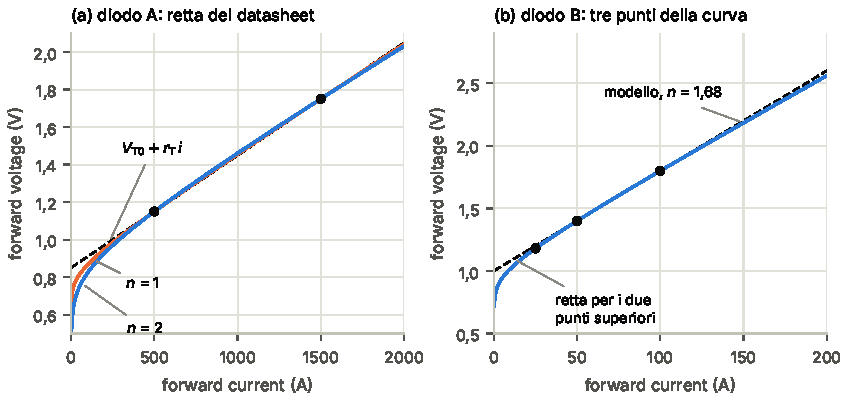
\includegraphics[width=\textwidth]{figures/fig_forward_it.pdf}
\caption{Forward characteristic del modello confrontata con i dati. (a) Diodo A: retta del datasheet (tratteggiata), con i suoi due punti, e il secant fit per $n = 1$ e $n = 2$. (b) Diodo B: fit su tre punti della curva, e la retta per i due punti superiori (tratteggiata).}
\label{fig:forward}
\end{figure}

\subsection{Verifica in una commutation cell simulata}
\label{sec:cell}
Il modello completo, con la junction capacitance, il leakage e la resistenza serie, è stato simulato nella cella della Fig.~\ref{fig:model}b con $L = \VR/a$ e uno snubber RC (Appendice~\ref{app:scripts}). Le junction capacitance sono stime, $\Cjo = \SI{\lmACj}{\nano\farad}$ per A e \SI{\lmBCj}{\nano\farad} per B. La Tabella~\ref{tab:cell} confronta la simulazione con le forme chiuse e la Fig.~\ref{fig:cell} mostra le forme d'onda.

\begin{table}[htb]
\centering\small
\caption{Commutation cell simulata confrontata con le forme chiuse. Le forme chiuse sono valutate al di/dt della simulazione; la carica è integrata fino al \SI{\lmPEndPct}{\percent} del picco, \eqref{eq:qrp}.}
\label{tab:cell}
\begin{tabular}{@{}lcc@{}}
\toprule
 & Diodo A & Diodo B \\
\midrule
Induttanza $L = \VR/a$ & \SI{\lmAL}{\micro\henry} & \SI{\lmBL}{\micro\henry} \\
Snubber $\Rsn$, $\Csn$ & \SI{\lmARsn}{\ohm}, \SI{\lmACsn}{\nano\farad} & \SI{\lmBRsn}{\ohm}, \SI{\lmBCsn}{\nano\farad} \\
di/dt allo zero della corrente & \SI{\lmASimSlope}{\ampere\per\micro\second} ($\lmASimSlopeErr\,\%$) & \SI{\lmBSimSlope}{\ampere\per\micro\second} ($\lmBSimSlopeErr\,\%$) \\
\addlinespace
$\Irr$, forma chiusa \eqref{eq:lambert} & \SI{\lmASimIrrCf}{\ampere} & \SI{\lmBSimIrrCf}{\ampere} \\
$\Irr$, simulazione, diffusion current & \SI{\lmASimIrrDif}{\ampere} ($\lmASimIrrDifErr\,\%$) & \SI{\lmBSimIrrDif}{\ampere} ($\lmBSimIrrDifErr\,\%$) \\
$\Irr$, simulazione, ai terminali & \SI{\lmASimIrrTerm}{\ampere} ($\lmASimIrrTermErr\,\%$) & \SI{\lmBSimIrrTerm}{\ampere} ($\lmBSimIrrTermErr\,\%$) \\
\addlinespace
$Q_\mathrm{r}$, forma chiusa \eqref{eq:qrp} & \SI{\lmASimQCf}{\micro\coulomb} & \SI{\lmBSimQCf}{\micro\coulomb} \\
$Q_\mathrm{r}$, simulazione, ai terminali & \SI{\lmASimQTerm}{\micro\coulomb} ($\lmASimQTermErr\,\%$) & \SI{\lmBSimQTerm}{\micro\coulomb} ($\lmBSimQTermErr\,\%$) \\
Carica della junction capacitance, \eqref{eq:qc} & \SI{\lmAQc}{\micro\coulomb} & \SI{\lmBQc}{\micro\coulomb} \\
\addlinespace
$\trr$, retta, forma chiusa \eqref{eq:trr} & \SI{\lmASimTrrCf}{\micro\second} & \SI{\lmBSimTrrCf}{\nano\second} \\
$\trr$, retta, simulazione & \SI{\lmASimTrr}{\micro\second} & \SI{\lmBSimTrr}{\nano\second} \\
\addlinespace
Peak reverse voltage senza snubber, \eqref{eq:vrm} & \SI{\lmAVpk}{\volt} & \SI{\lmBVpk}{\volt} \\
Peak reverse voltage, simulazione con snubber & \SI{\lmASimVpk}{\volt} & \SI{\lmBSimVpk}{\volt} \\
Energia nel diodo dopo lo zero della corrente & \SI{\lmASimEd}{\milli\joule} & \SI{\lmBSimEd}{\milli\joule} \\
Energia nel resistore dello snubber & \SI{\lmASimEr}{\milli\joule} & \SI{\lmBSimEr}{\milli\joule} \\
Somma & \SI{\lmASimEsum}{\milli\joule} & \SI{\lmBSimEsum}{\milli\joule} \\
Bilancio $\VR\Qrr + \Csn\VR^2/2$, \eqref{eq:ebal} & \SI{\lmASimEbal}{\milli\joule} & \SI{\lmBSimEbal}{\milli\joule} \\
\bottomrule
\end{tabular}
\end{table}

La tabella mostra quattro cose.
\begin{itemize}
\item Il di/dt allo zero della corrente è un po' sopra $\VR/L$, perché la forward voltage del diodo si somma a $\VR$ mentre la corrente scende. L'effetto è qui inferiore all'uno per cento; cresce quando $\VR$ è piccola.
\item La diffusion current della simulazione segue la forma chiusa entro lo \SI{0.5}{\percent}. La corrente ai terminali è più alta al picco, dello \SI{0.1}{\percent} per A e dell'\SI{1.5}{\percent} per B: è la corrente della junction capacitance mentre la tensione sale. Per il diodo B la carica ai terminali supera la forma chiusa dello \SI{0.3}{\percent}, che è la carica della junction capacitance, come dice la nota della norma. Per il diodo A quella carica è trascurabile, e lo \SI{0.1}{\percent} che resta viene dal di/dt, che non è esattamente costante lungo la rampa perché la forward voltage cambia con la corrente.
\item Il recovery time della convenzione della retta è riprodotto entro lo \SI{0.6}{\percent}.
\item Il bilancio dell'energia \eqref{eq:ebal} si chiude entro lo \SI{0.5}{\percent}. Per il diodo A lo snubber è rapido rispetto alla tail ($\Rsn\Csn = \SI{\lmARsnCsn}{\micro\second}$, $\taurr = \SI{\lmATrr}{\micro\second}$): arrotonda il gradino della tensione, ma il picco è \SI{\lmASimVpk}{\volt}, praticamente i \SI{\lmAVpk}{\volt} che la \eqref{eq:vrm} dà per il solo diodo, e quasi tutta l'energia resta nel diodo. Per il diodo B lo snubber è lento quanto la tail ($\Rsn\Csn = \SI{\lmBRsnCsn}{\nano\second}$, $\taurr = \SI{\lmBTrr}{\nano\second}$): abbassa il picco da \SI{\lmBVpk}{\volt} a \SI{\lmBSimVpk}{\volt} e prende più di metà dell'energia.
\end{itemize}

\begin{figure}[htb]
\centering
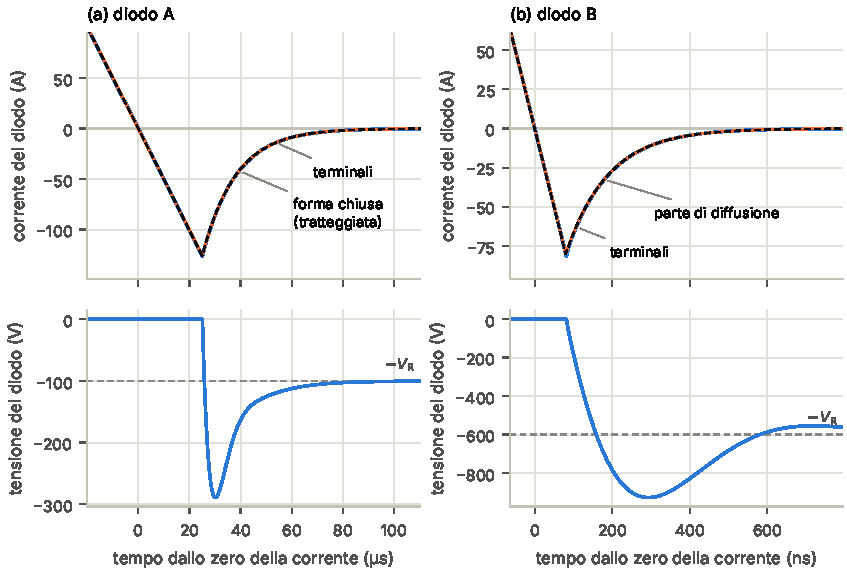
\includegraphics[width=\textwidth]{figures/fig_cell_it.pdf}
\caption{Commutation cell simulata con lo snubber: corrente e tensione del diodo. La corrente ai terminali, la diffusion current e la forma chiusa della Sez.~\ref{sec:ramp} (tratteggiata) si sovrappongono; per il diodo B la corrente ai terminali è leggermente sopra la diffusion current al picco, della corrente della junction capacitance.}
\label{fig:cell}
\end{figure}

\subsection{Lontano dal punto del datasheet}
\label{sec:away}
La Tabella~\ref{tab:awaya} e la Fig.~\ref{fig:curves} mostrano i due set ad altri di/dt e forward current.

\begin{table}[htb]
\centering\small
\caption{Diodo A lontano dal punto del datasheet, a $\IF = \SI{\lmAIf}{\ampere}$: il set della Tabella~\ref{tab:conv} confrontato con la curva ipotetica del datasheet, e il set che la curva richiede a ogni di/dt (punto della curva convertito con la softness del punto del datasheet).}
\label{tab:awaya}
\begin{tabular}{@{}lccccc@{}}
\toprule
di/dt $a$ [\si{\ampere\per\micro\second}] & \lmAAwayALo & \lmAAwayALoB & \lmAAwayARef & \lmAAwayAHiB & \lmAAwayAHi \\
\midrule
Durata della rampa, $x = \Tone/\tau$ & \lmAAwayXALo & \lmAAwayXALoB & \lmAAwayXARef & \lmAAwayXAHiB & \lmAAwayXAHi \\
$\Irr$ del set [A] & \lmAAwayIrrALo & \lmAAwayIrrALoB & \lmAAwayIrrARef & \lmAAwayIrrAHiB & \lmAAwayIrrAHi \\
$\Qrr$ del set [\si{\micro\coulomb}] & \lmAAwayQrrALo & \lmAAwayQrrALoB & \lmAAwayQrrARef & \lmAAwayQrrAHiB & \lmAAwayQrrAHi \\
$\Qrr$ della curva del datasheet [\si{\micro\coulomb}] & \lmAAwayDsALo & \lmAAwayDsALoB & \lmAAwayDsARef & \lmAAwayDsAHiB & \lmAAwayDsAHi \\
Set rispetto alla curva & \lmAAwayRatioALo & \lmAAwayRatioALoB & \lmAAwayRatioARef & \lmAAwayRatioAHiB & \lmAAwayRatioAHi \\
\addlinespace
Punto della curva convertito: $\tau$ [\si{\micro\second}] & \lmAAwayTauALo & \lmAAwayTauALoB & \lmAAwayTauARef & \lmAAwayTauAHiB & \lmAAwayTauAHi \\
Punto della curva convertito: $\TM$ [\si{\micro\second}] & \lmAAwayTmALo & \lmAAwayTmALoB & \lmAAwayTmARef & \lmAAwayTmAHiB & \lmAAwayTmAHi \\
\bottomrule
\end{tabular}
\end{table}

Per il diodo A il set è su una rampa lunga fino a circa \SI{10}{\ampere\per\micro\second}: la sua carica è proporzionale al di/dt, mentre la curva del datasheet cresce con l'esponente \num{\lmAQexp}. Una decade sotto il punto del datasheet il set ha un quinto della carica della curva. Le ultime due righe sono i set che riproducono la curva a ogni di/dt: il lifetime va da \SI{\lmAAwayTauALo}{\micro\second} al di/dt più basso a \SI{\lmAAwayTauAHi}{\micro\second} al più alto, seguendo la \eqref{eq:taucurve} finché la rampa è lunga. Al di/dt del datasheet la forward current non ha quasi effetto: \SI{\lmAAwayQrrFLo}{\micro\coulomb} a \SI{\lmAAwayFLo}{\ampere} e \SI{\lmAAwayQrrFHi}{\micro\coulomb} a \SI{\lmAAwayFHi}{\ampere}, contro \SI{\lmAQrr}{\micro\coulomb} a \SI{\lmAIf}{\ampere}.

Il diodo B si comporta in modo opposto. A di/dt doppio la carica cresce da \SI{\lmBQrr}{\micro\coulomb} a soli \SI{\lmBAwayQrrAHi}{\micro\coulomb}, e a metà di/dt scende a \SI{\lmBAwayQrrALo}{\micro\coulomb}; a forward current doppia è \SI{\lmBAwayQrrFHi}{\micro\coulomb} e a metà forward current \SI{\lmBAwayQrrFLo}{\micro\coulomb}. La corrente di picco va da \SI{\lmBAwayIrrALo}{\ampere} a \SI{\lmBAwayIrrAHi}{\ampere} sui due di/dt e da \SI{\lmBAwayIrrFLo}{\ampere} a \SI{\lmBAwayIrrFHi}{\ampere} sulle due correnti. Il punto a metà di/dt e il punto a forward current doppia hanno lo stesso rapporto $\IF/a$, e il secondo vale il doppio del primo, nel picco e nella carica: è l'omogeneità della Sez.~\ref{sec:exponents}.

\begin{figure}[htb]
\centering
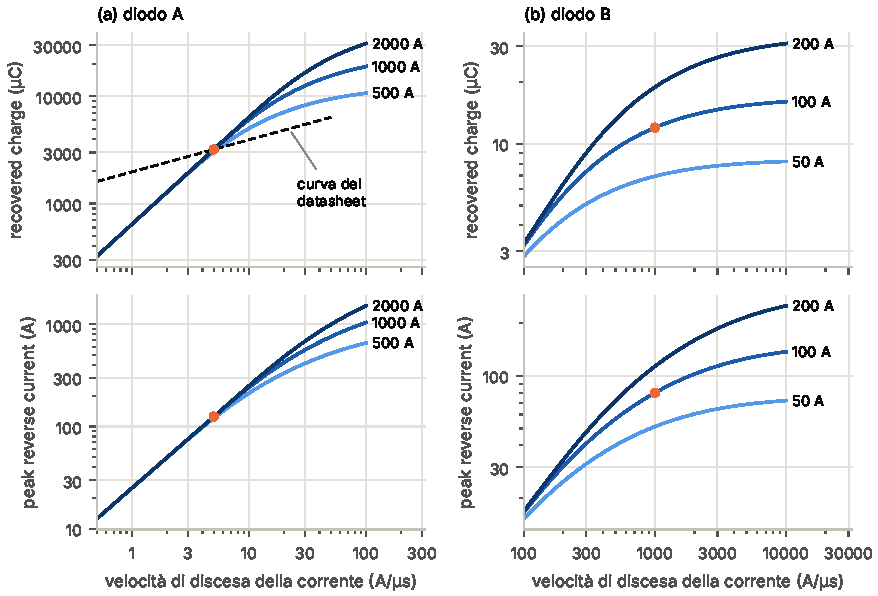
\includegraphics[width=\textwidth]{figures/fig_curves_it.pdf}
\caption{I due set della Tabella~\ref{tab:conv} ad altri di/dt, per metà, una e due volte la forward current della prova del datasheet. Il punto è il punto del datasheet. Per il diodo A la linea tratteggiata è la curva ipotetica del datasheet.}
\label{fig:curves}
\end{figure}

\subsection{Temperatura}
Per il diodo B il datasheet fornisce il recovery anche a \SI{\lmBTtwo}{\celsius}. La stessa conversione dà $\taurr = \SI{\lmBTrrTtwo}{\nano\second}$, $\tau = \SI{\lmBTauTtwo}{\nano\second}$ e $\TM = \SI{\lmBTmTtwo}{\nano\second}$: rispetto a \SI{\lmBT}{\celsius} il lifetime è più basso del \SI{\lmBTauTtwoPct}{\percent} e il transit time del \SI{\lmBTmTtwoPct}{\percent}. I due parametri non scalano insieme, quindi anche la softness cambia con la temperatura.

Per il diodo A non ci sono dati a una seconda temperatura. Come esempio della scalatura \eqref{eq:scale}, un set con entrambe le costanti di tempo più basse del \SI{\lmAIrrTtwoPct}{\percent} ($\tau = \SI{\lmATauTtwo}{\micro\second}$, $\TM = \SI{\lmATmTtwo}{\micro\second}$) dà al di/dt del datasheet $\Irr = \SI{\lmAIrrTtwo}{\ampere}$ e $\Qrr = \SI{\lmAQrrTtwo}{\micro\coulomb}$: il picco scende dello stesso \SI{\lmAIrrTtwoPct}{\percent} e la carica del \SI{\lmAQrrTtwoPct}{\percent}, perché va con il quadrato delle costanti di tempo. Nell'altro senso, una carica nota per essere più bassa del \SI{\lmAQrrTtwoPct}{\percent} a una temperatura più bassa richiede costanti di tempo più basse del \SI{\lmAIrrTtwoPct}{\percent}.

\subsection{Gli stessi diodi in altre descrizioni}
\begin{table}[htb]
\centering\small
\caption{Grandezze dei due set in altre convenzioni e circuiti di prova.}
\label{tab:other}
\begin{tabular}{@{}llcc@{}}
\toprule
Grandezza & & Diodo A & Diodo B \\
\midrule
$\trr$, retta per il \SI{90}{\percent} e il \SI{25}{\percent} & \eqref{eq:trr} & \SI{\lmATrrLine}{\micro\second} & \SI{\lmBTrrLine}{\nano\second} \\
$\trr$, corrente al \SI{10}{\percent} del picco & \eqref{eq:trr} & \SI{\lmATrrTen}{\micro\second} & \SI{\lmBTrrTen}{\nano\second} \\
$\trr$, triangolo di uguale carica, $2\Qrr/\Irr$ & & \SI{\lmATrrTri}{\micro\second} & \SI{\lmBTrrTri}{\nano\second} \\
Stretch factor $\trr\,a/\Irr$ (convenzione del \SI{10}{\percent}) & & \lmAStretch & \lmBStretch \\
$\tb/\ta$, convenzione della retta & & \lmASLine & \lmBSLine \\
\addlinespace
Commutazione brusca: $\Irr = \IF\tau/\TM$ & \eqref{eq:abrupt} & \SI{\lmAIrrFast}{\ampere} & \SI{\lmBIrrFast}{\ampere} \\
Commutazione brusca: $\Qrr = \IF(\tau-\taurr)$ & \eqref{eq:abrupt} & \SI{\lmAQrrFast}{\micro\coulomb} & \SI{\lmBQrrFast}{\micro\coulomb} \\
Carica statica rispetto alla carica del datasheet, $\tau\IF/\Qrr$ & & \lmATauIfRatio & \lmBTauIfRatio \\
\addlinespace
Peak reverse voltage senza snubber, $\VR(1+2/s)$ & \eqref{eq:vrm} & \SI{\lmAVpk}{\volt} & \SI{\lmBVpk}{\volt} \\
Energia di recovery $\VR\,\Qrr$ & \eqref{eq:erec} & \SI{\lmAErec}{\milli\joule} & \SI{\lmBErec}{\milli\joule} \\
\bottomrule
\end{tabular}
\end{table}

La Tabella~\ref{tab:other} riporta i due set nelle altre convenzioni della Sez.~\ref{sec:direct}. Altri due circuiti di prova completano il quadro.

\emph{Commutazione resistiva del diodo B.} Con $\IF = \SI{\lmBStepIf}{\ampere}$ e $\IR = \SI{\lmBStepIr}{\ampere}$ il rapporto $\IF/\IR = \lmBStepRatio$ è sotto $\TM/\tau = \lmBTmOverTau$: non c'è fase di storage. La reverse current parte da $\IF\tau/\TM = \SI{\lmBStepIzero}{\ampere}$ e scende a \SI{\lmBStepIrec}{\ampere} in \SI{\lmBStepTrr}{\nano\second}. Con $\IF = \SI{\lmBStepIfTwo}{\ampere}$ lo storage time \eqref{eq:ts} è \SI{\lmBStepTsTwo}{\nano\second} e la corrente raggiunge \SI{\lmBStepIrec}{\ampere} dopo \SI{\lmBStepTrrTwo}{\nano\second}. Un recovery time misurato in una prova di questo tipo ha poco a che fare con i \SI{\lmBTrrLine}{\nano\second} della prova su rampa, e dipende dalle due correnti della prova.

\emph{Impulso semisinusoidale sul diodo A.} Una semisinusoide di \SI{\lmASineLongMs}{\milli\second} con il di/dt del datasheet al suo zero ha un picco di \SI{\lmASineLongIpk}{\kilo\ampere}; la \eqref{eq:sine} dà una peak reverse current entro il $\lmASineLongErr\,\%$ del valore per rampa lunga $a(\tau-\taurr) = \SI{\lmALongIrr}{\ampere}$. Con una semisinusoide di \SI{\lmASineShortMs}{\milli\second} (picco \SI{\lmASineShortIpk}{\kilo\ampere}, $\omega\tau = \lmASineShortWt$) la differenza è $\lmASineShortErr\,\%$. Per il modello, una prova semisinusoidale a frequenza di rete e una prova su rampa con lo stesso di/dt allo zero sono la stessa prova.

\subsection{Sensibilità delle due conversioni}
\begin{table}[htb]
\centering\small
\caption{Variazione relativa dei parametri della conversione esatta per una variazione relativa di un dato dell'uno per cento (derivate numeriche di \eqref{eq:taurr}, \eqref{eq:iter} e \eqref{eq:tm}).}
\label{tab:sensex}
\begin{tabular}{@{}lcccccc@{}}
\toprule
 & \multicolumn{3}{c}{Diodo A} & \multicolumn{3}{c}{Diodo B} \\
\cmidrule(lr){2-4}\cmidrule(l){5-7}
Dato & $\tau$ & $\taurr$ & $\TM$ & $\tau$ & $\taurr$ & $\TM$ \\
\midrule
$\Qrr$ & $\lmASensTauQ$ & $\lmASensTrrQ$ & $\lmASensTmQ$ & $\lmBSensTauQ$ & $\lmBSensTrrQ$ & $\lmBSensTmQ$ \\
$\Irr$ & $\lmASensTauI$ & $\lmASensTrrI$ & $\lmASensTmI$ & $\lmBSensTauI$ & $\lmBSensTrrI$ & $\lmBSensTmI$ \\
$a$ & $\lmASensTauA$ & $\lmASensTrrA$ & $\lmASensTmA$ & $\lmBSensTauA$ & $\lmBSensTrrA$ & $\lmBSensTmA$ \\
$\IF$ & $\lmASensTauF$ & $\lmASensTrrF$ & $\lmASensTmF$ & $\lmBSensTauF$ & $\lmBSensTrrF$ & $\lmBSensTmF$ \\
\bottomrule
\end{tabular}
\end{table}
Per il diodo A i numeri della Tabella~\ref{tab:sensex} sono quelli della \eqref{eq:sens} con $s = \lmAS$ entro \num{0.01}, e la forward current non ha peso. Una corrente di picco più alta del \SI{5}{\percent} a parità di carica sposta $\tau$ del $\lmAFiveTau\,\%$, $\taurr$ del $\lmAFiveTrr\,\%$ e $\TM$ del $\lmAFiveTm\,\%$. Per il diodo B la stessa variazione dà $\lmBFiveTau\,\%$, $\lmBFiveTrr\,\%$ e $\lmBFiveTm\,\%$. Sulla sua rampa corta il lifetime dipende dalla forward current della prova quasi quanto dalla corrente di picco, e poco dal di/dt: la forward current della prova del datasheet va conosciuta e usata.

%=====================================================================
\section{Procedura}
\label{sec:procedure}
\begin{enumerate}
\item \emph{Scegliere i dati.} Prendere $\Irr$ e $\Qrr$ alla temperatura di interesse e al di/dt più vicino a quello dell'applicazione, con la forward current, il di/dt e la reverse voltage della prova. Annotare se sono valori massimi o tipici e quale convenzione definisce il recovery time, se lo si usa (Tabella~\ref{tab:kappa}).
\item \emph{Verificare la coppia.} La carica deve superare il triangolo: $\Qrr > \Irr^2/(2a)$. Calcolare $\Irr/\IF$: sotto \num{0.1} la rampa della prova è lunga; sopra, può non esserlo (Tabella~\ref{tab:valid}).
\item \emph{Tail time constant.} $\taurr = \Qrr/\Irr - \Irr/(2a)$, \eqref{eq:taurr}; da altre coppie, da \eqref{eq:fromtrr} a \eqref{eq:fromq}.
\item \emph{Lifetime.} Iterare \eqref{eq:iter} a partire da $\tau = \taurr + \Irr/a$. Su una rampa lunga il valore di partenza è il risultato.
\item \emph{Transit time.} $\TM = \tau\taurr/(\tau-\taurr)$, \eqref{eq:tm}. La softness del diodo su una rampa lunga è $2\TM/\tau$.
\item \emph{Conduzione.} Scegliere $n$ (2 per un diodo di potenza in high injection) e fare il fit di $\IS$ e $\RS$ sulla retta, \eqref{eq:tangent} o \eqref{eq:secant}, oppure il fit di tutti e tre su punti della curva, \eqref{eq:points}. Moltiplicare $\IS$ per $(\tau+\TM)/\tau$ se l'implementazione scrive la junction law con $\tau\,\IS^{*}$.
\item \emph{Blocco.} $\Rr$ dalla reverse current alla tensione e alla temperatura di lavoro; $\Cjo$ dal datasheet o da una stima, \eqref{eq:cj}.
\item \emph{Verificare.} Riportare il set sulla rampa di prova, con \eqref{eq:lambert} o con una simulazione della cella di prova, e confrontare $\Irr$, $\Qrr$ e $\trr$ con il datasheet. Guardare poi il punto di lavoro dell'applicazione: di/dt, forward current e durata della rampa in lifetime. Se il di/dt è lontano da quello dei dati, convertire di nuovo dal punto più vicino della curva del datasheet (Sez.~\ref{sec:slope}).
\item \emph{Delimitare.} Dove il risultato dipende dalla softness (tensione di picco, smorzamento) o dallo spread tra i dispositivi, ripetere con $\TM$ agli estremi del suo intervallo (Sez.~\ref{sec:sens}) e con il set scalato \eqref{eq:scale}.
\end{enumerate}

%=====================================================================
\appendix
\section{Da dove vengono le due cariche}
\label{app:lumped}
Questa appendice dà una breve derivazione delle equazioni del modello, per mostrare che cosa rappresentano le due cariche e il transit time. Segue l'idea delle lumped charge di \cite{linvill1958} che \cite{lauritzen1991} applica al diodo; la scelta del profilo qui sotto è un modo di farlo, non una citazione dell'articolo.

\subsection*{Equazione del controllo di carica}
Si consideri la base debolmente drogata di un diodo p\textsuperscript{+}--n\textsuperscript{--}--n\textsuperscript{+}, di larghezza $2d$ e area $A$, in high injection: elettroni e lacune hanno la stessa concentrazione $p(x,t)$, che obbedisce all'equazione di diffusione ambipolare
\begin{equation}
\frac{\partial p}{\partial t} = D\,\frac{\partial^2 p}{\partial x^2} - \frac{p}{\tau} , \qquad -d \leq x \leq d ,
\label{eq:diffusion}
\end{equation}
con l'ambipolar diffusion constant $D$ e l'high-injection lifetime $\tau$. Con emettitori ideali la corrente entra come gradiente della concentrazione ai due bordi; per mobilità uguali di elettroni e lacune, $i = 2qAD\,\partial p/\partial x$ in $x = d$ e il gradiente opposto in $x = -d$. Integrando \eqref{eq:diffusion} sulla base, con la stored charge $Q = qA\int p\,\diff x$, si ottiene
\begin{equation}
\frac{\diff Q}{\diff t} = i - \frac{Q}{\tau} .
\label{eq:cc}
\end{equation}
È l'equazione del controllo di carica, ed è esatta. È la \eqref{eq:qm} se la middle charge è l'intera stored charge, $\qM = Q$. Ciò che non dice è come la corrente dipenda dallo stato della base: per questo serve la forma del profilo.

\subsection*{Due lumped charge}
Si descriva il profilo con due numeri, la concentrazione $p_\mathrm{E}$ ai bordi e $p_\mathrm{M}$ al centro, raccordati da una parabola: $p(x) = p_\mathrm{M} + (p_\mathrm{E}-p_\mathrm{M})\,(x/d)^2$. Allora il gradiente al bordo è $2\,(p_\mathrm{E}-p_\mathrm{M})/d$ e la stored charge è $Q = \tfrac{2}{3}\,qAd\,(2p_\mathrm{M}+p_\mathrm{E})$. Si definisca l'edge charge come la carica che la base conterrebbe se la concentrazione di bordo la riempisse, $\qE = 2qAd\,p_\mathrm{E}$. Allora $\qE - \qM = \tfrac43\,qAd\,(p_\mathrm{E}-p_\mathrm{M})$ e la corrente è
\begin{equation}
i = \frac{4qAD\,(p_\mathrm{E}-p_\mathrm{M})}{d} = \frac{\qE-\qM}{\TM} , \qquad \TM = \frac{d^2}{3D} .
\label{eq:tmgeom}
\end{equation}
È la \eqref{eq:idif}: la corrente è la diffusione dai bordi verso il centro, e il transit time è il tempo di diffusione sulla semilarghezza della base.

\subsection*{Legge di giunzione}
In high injection il prodotto delle concentrazioni dei portatori ai due bordi della base segue la somma $\vj$ delle due tensioni di giunzione, $p_\mathrm{E}^2 = n_\mathrm{i}^2\,e^{\vj/\VT}$ per un profilo simmetrico, quindi $p_\mathrm{E} = n_\mathrm{i}\,e^{\vj/(2\VT)}$: l'edge charge segue la junction voltage con l'emission coefficient $n = 2$. È la \eqref{eq:qe}. Una reverse voltage porta a zero la concentrazione di bordo e non può fare di più: è la giunzione interdetta, $\qE = 0$, della Sez.~\ref{sec:regimes}.

\subsection*{Quanto può fare un solo numero}
Il transit time della \eqref{eq:tmgeom} viene da un profilo, e altri stati della base richiedono altri valori. In regime stazionario il profilo esatto di \eqref{eq:diffusion} è un coseno iperbolico, e il rapporto tra l'edge charge e la stored charge dà
\begin{equation}
\frac{\TM}{\tau} = \frac{d}{L}\,\coth\frac{d}{L} - 1 , \qquad L = \sqrt{D\,\tau} ,
\label{eq:tmstatic}
\end{equation}
che vale $d^2/(3D\tau)$ per una base più stretta della diffusion length $L$, il valore della \eqref{eq:tmgeom}. Dopo l'interdizione, con la concentrazione mantenuta a zero a entrambi i bordi, il modo più lento di \eqref{eq:diffusion} è un coseno che decade con la velocità $1/\tau + \pi^2 D/(4d^2)$; confrontato con $1/\taurr = 1/\tau + 1/\TM$ richiede $\TM = 4d^2/(\pi^2 D)$, che è il \SI{22}{\percent} sopra la \eqref{eq:tmgeom}. Il transit time è quindi dell'ordine di $d^2/(3D)$, ma non è una costante calcolabile dalla geometria: è un parametro efficace, da ricavare dalla forma d'onda di recovery.

L'ordine di grandezza resta comunque una verifica utile di una conversione. Con un'ambipolar diffusion constant di \SI{\lmADcm}{\centi\metre\squared\per\second}, un valore indicativo per il silicio a \SI{\lmAT}{\celsius} [M] \cite{lutz}, il transit time del diodo A corrisponde a una larghezza di base $2d$ di \SI{\lmAWpar}{\micro\metre} con la \eqref{eq:tmgeom}, \SI{\lmAWmode}{\micro\metre} con il modo più lento e \SI{\lmAWstat}{\micro\metre} con la \eqref{eq:tmstatic}; la diffusion length è \SI{\lmALdiff}{\micro\metre}. Circa mezzo millimetro è una base plausibile per un diodo da \SI{\lmAVrrmKv}{\kilo\volt} [M]. Per il diodo B, con \SI{\lmBDcm}{\centi\metre\squared\per\second}, le stesse tre relazioni danno \SI{\lmBWpar}{\micro\metre}, \SI{\lmBWmode}{\micro\metre} e \SI{\lmBWstat}{\micro\metre}. I dati di entrambi i diodi sono ipotetici, quindi questi numeri non dicono nulla su componenti reali; mostrano come si legge la verifica. Su un datasheet reale una larghezza lontana da ciò che suggerisce la classe di tensione significa che i due parametri sono behavioural: riproducono la forma d'onda di prova, non l'interno del dispositivo. In qualche misura è sempre così, perché una base reale non è simmetrica: elettroni e lacune hanno mobilità diverse, e la carica è rimossa prima dal lato p\textsuperscript{+}.

%=====================================================================
\section{Dimostrazioni}
\label{app:proofs}
\subsection{Forma chiusa del picco}
\label{app:lambert}
Si scriva la prima delle \eqref{eq:norm} come $y = c - c\,e^{-\lambda}e^{-y}$ con $c = 1-\rho$, e si ponga $w = y - c$. Allora $w = -c\,e^{-(\lambda+c)}\,e^{-w}$, cioè
\begin{equation}
w\,e^{w} = -c\,e^{-(\lambda+c)} .
\end{equation}
Il secondo membro è compreso tra $-1/e$ e zero, perché $c\,e^{-c} \leq 1/e$. Poiché $0 < y < c < 1$, $w$ è compreso tra $-1$ e zero, che è il codominio del ramo principale: $w = W_0(-c\,e^{-(\lambda+c)})$, e segue la \eqref{eq:lambert}.

\subsection{Convergenza dell'iterazione}
\label{app:contraction}
Sia $g(\tau) = \taurr + \ta/(1-e^{-\Tone/\tau})$ il secondo membro della \eqref{eq:iter}, per $\tau > 0$. Con $x = \Tone/\tau$ la sua derivata è
\begin{equation}
g'(\tau) = \frac{\ta}{\Tone}\,\frac{x^2\,e^{-x}}{(1-e^{-x})^2} = \frac{\ta}{\Tone}\left(\frac{x/2}{\sinh(x/2)}\right)^{2} .
\end{equation}
La parentesi è compresa tra zero e uno, quindi
\begin{equation}
0 < g'(\tau) < \frac{\ta}{\Tone} = \frac{\Irr}{\IF+\Irr} < 1 .
\end{equation}
La mappa $g$ è una contrazione sull'intera semiretta: ha un solo punto fisso, l'iterazione vi converge da qualunque valore di partenza, e a ogni passo l'errore si riduce di un fattore minore di $\Irr/(\IF+\Irr)$. Poiché $g$ è crescente e $g(\taurr+\ta) > \taurr+\ta$, la successione che parte dalla forma chiusa sale in modo monotono verso la soluzione: la forma chiusa sottostima sempre il lifetime. Su una rampa lunga la parentesi è molto piccola e bastano due o tre passi; quando $\Irr$ è vicina a $\IF$ e la rampa è corta il fattore è vicino a un mezzo. La soluzione esiste per ogni $\taurr > 0$, quindi l'unica condizione sui dati è $\Qrr > \Irr^2/(2a)$. Il transit time \eqref{eq:tm} è positivo perché la soluzione ha $\tau > \taurr + \ta$.

\subsection{Esponenti}
\label{app:exponents}
Derivando la prima delle \eqref{eq:norm} rispetto a $\lambda$, con $(1-\rho)\,e^{-(\lambda+y)} = 1-\rho-y$, si ottiene
\begin{equation}
\frac{\diff y}{\diff\lambda} = \frac{1-\rho-y}{\rho+y} .
\end{equation}
Con $\Irr = a\tau\,y(\lambda)$ e $\lambda = \IF/(a\tau)$, $\partial\ln\Irr/\partial\ln a = 1 - (\lambda/y)\,\diff y/\diff\lambda$, che è la prima delle \eqref{eq:exponents}; la seconda segue allo stesso modo da $\Qrr = a\tau^2\,(y^2/2+\rho y)$. Le derivate rispetto a $\ln\IF$ sono $(\lambda/y)\,\diff y/\diff\lambda$ e la sua omologa per la carica, quindi le somme valgono uno, \eqref{eq:euler}.

%=====================================================================
\section{Script}
\label{app:scripts}
Accanto a questa nota si trovano due file Python. Richiedono solo NumPy, SciPy e Matplotlib.
\begin{itemize}
\emergencystretch=3em
\item \texttt{lm\_conversion.py} è un modulo con le relazioni della nota in unità SI: la soluzione su rampa (\texttt{ramp\_recovery}, \texttt{ramp\_peak\_norm}, \texttt{ramp\_exponents}, \texttt{ramp\_waveform}), le convenzioni del recovery time (\texttt{trr\_factor}), gli altri circuiti di prova (\texttt{step\_recovery}, \texttt{sine\_peak}), le conversioni (\texttt{lm\_from\_irr\_qrr}, \texttt{lm\_from\_irr\_trr}, \texttt{irr\_from\_qrr\_trr}, \texttt{irr\_from\_qrr\_softness}, \texttt{sensitivities}), i fit della forward characteristic (\texttt{forward\_tangent}, \texttt{forward\_secant}, \texttt{forward\_points}), la junction capacitance, e la simulazione della commutation cell con gli strumenti per leggere una forma d'onda come farebbe un datasheet (\texttt{simulate\_cell}, \texttt{measure}). Eseguito come programma verifica le forme chiuse con un'integrazione passo passo.
\item \texttt{lm\_conversion\_calc.py} contiene in testa i dati dei due diodi e produce i numeri e le figure della nota: il log \texttt{lm\_conversion\_results.txt}, il file \texttt{lm\_conversion\_values.tex} con ogni numero citato qui come macro, letto da entrambe le versioni linguistiche, e \texttt{figures/*.pdf} (le figure con etichette italiane sono \texttt{figures/*\_it.pdf}). Viene eseguito in pochi secondi. Per convertire un altro diodo, sostituire i dati di uno dei due dizionari.
\end{itemize}

\emph{Commutation cell.} La cella della Fig.~\ref{fig:model}b ha quattro stati: la corrente $i_\mathrm{sw}$ dell'interruttore, la middle charge, la junction voltage e la tensione $v_\mathrm{c}$ del condensatore dello snubber,
\begin{equation}
\begin{aligned}
L\,\frac{\diff i_\mathrm{sw}}{\diff t} &= \VR + v , &\qquad \frac{\diff\qM}{\diff t} &= \frac{\qE-\qM}{\TM} - \frac{\qM}{\tau} , \\
\Cj(\vj)\,\frac{\diff\vj}{\diff t} &= i - \frac{\qE-\qM}{\TM} - \frac{\vj}{\Rr} , &\qquad \Csn\,\frac{\diff v_\mathrm{c}}{\diff t} &= \frac{v - v_\mathrm{c}}{\Rsn} ,
\end{aligned}
\end{equation}
con $i = \IF - i_\mathrm{sw} - (v-v_\mathrm{c})/\Rsn$, $v = \vj + \RS\,i$ e $\qE$ dalla \eqref{eq:qe}. Il sistema è rigido (\emph{stiff}), perché la junction voltage reagisce molto più rapidamente della carica; è integrato con un metodo implicito (Radau, tolleranza relativa $10^{-9}$) e lo Jacobiano analitico. La forma d'onda viene poi letta come in una prova: di/dt subito prima dello zero della corrente, picco, carica fino al \SI{\lmPEndPct}{\percent} del picco, recovery time con la retta.

%=====================================================================
\begin{thebibliography}{99}
\small
\item[] I riferimenti contrassegnati con [M] sono citati a memoria: i loro dati bibliografici, e le affermazioni tratte da essi, vanno verificati sulla fonte prima dell'uso in un documento di progetto. Gli altri sono stati letti, o ne sono stati verificati i dati bibliografici, quando la nota è stata scritta; la documentazione dei simulatori è stata letta sul web nel novembre 2026. I titoli sono riportati nella lingua originale.

\bibitem{lauritzen1991}
P.~O.~Lauritzen, C.~L.~Ma, ``A simple diode model with reverse recovery'', \emph{IEEE Trans. Power Electron.}, vol.~6, n.~2, pp.~188--191, apr.~1991. doi:\,10.1109/63.76804.

\bibitem{ma1993}
C.~L.~Ma, P.~O.~Lauritzen, ``A simple power diode model with forward and reverse recovery'', \emph{IEEE Trans. Power Electron.}, vol.~8, n.~4, pp.~342--346, ott.~1993. doi:\,10.1109/63.261002.

\bibitem{linvill1958}
J.~G.~Linvill, ``Lumped models of transistors and diodes'', \emph{Proc. IRE}, vol.~46, n.~6, pp.~1141--1152, giugno~1958. doi:\,10.1109/JRPROC.1958.286896.

\bibitem{pemodels}
University of Washington, Department of Electrical Engineering, pagine web sui modelli di dispositivi a semiconduttore di potenza: \emph{Basic Diode with Reverse Recovery}, aggiornata il 23~gennaio 2013, \url{https://labs.ece.uw.edu/pemodels/modtext/diode-b.html}, e la pagina del diodo con forward e reverse recovery, \url{https://labs.ece.uw.edu/pemodels/modtext/diode-fr.html}.

\bibitem{iec60747}
IEC~60747-2:2025, \emph{Semiconductor devices -- Part~2: Discrete devices -- Rectifier diodes}, Ed.~4.0, settembre 2025. Le definizioni 3.3.10 (peak reverse recovery current), 3.5.2 (reverse recovery time), 3.5.3 e 3.5.4 (rise time e fall time), 3.5.5 (recovered charge) sono state lette nell'anteprima pubblica della norma. Il punto 6.3.5 (metodi di misura) è citato dall'indice; le definizioni della threshold voltage e della slope resistance non sono state lette.

\bibitem{an6481}
Dynex Semiconductor, \emph{RC Snubber Design for Dynex Thyristors and Diodes}, Application Note AN6481-1, LN43754, novembre 2024. Sez.~2.1 (forma d'onda del reverse recovery, recovery time con la retta per il \SI{90}{\percent} e il \SI{25}{\percent} del picco, softness), Sez.~2.2, Eqq.~(1) e~(2) (tail esponenziale e sua costante di tempo).

\bibitem{an5028}
STMicroelectronics, \emph{Calculation of turn-off power losses generated by an ultrafast diode}, Application Note AN5028, Rev.~1, ottobre 2017. Definizioni del recovery time, della frazione $k$ e della softness.

\bibitem{an5950}
D.~Chamund, C.~Rout, \emph{Understanding i\textsuperscript{2} Phase Control Thyristor Datasheets}, Dynex Semiconductor, Application Note AN5950-1, LN26885, settembre 2009. Figg.~12 e~13 (stored charge e reverse current in funzione del di/dt).

\bibitem{mathworks}
MathWorks, documentazione di Simscape Electrical, pagina di riferimento del blocco \emph{Diode}, release R2026b, sezioni ``Charge Dynamics'', ``How the Block Calculates TM and tau'' e ``Alternatives to Specifying trr Directly''. \url{https://www.mathworks.com/help/sps/ref/diode.html}.

\bibitem{plecs}
Plexim, documentazione di PLECS, versione 5.0, componente \emph{Diode with Reverse Recovery}. \url{https://docs.plexim.com/plecs/5.0/components-by-category/rrdiode/}.

\bibitem{schlangenotto1969}
H.~Schlangenotto, W.~Gerlach, ``On the effective carrier lifetime in p-s-n rectifiers at high injection levels'', \emph{Solid-State Electronics}, vol.~12, n.~4, pp.~267--275, 1969. doi:\,10.1016/0038-1101(69)90008-2.

\bibitem{nagel1975}
[M] L.~W.~Nagel, \emph{SPICE2: A computer program to simulate semiconductor circuits}, Memorandum ERL-M520, University of California, Berkeley, 1975. Modello di diodo con il transit time \texttt{TT}.

\bibitem{lutz}
[M] J.~Lutz, H.~Schlangenotto, U.~Scheuermann, R.~De~Doncker, \emph{Semiconductor Power Devices: Physics, Characteristics, Reliability}, Springer, 2011. Carrier lifetime, diffusione ambipolare, reverse recovery, reverse current.

\end{thebibliography}

\end{document}
